% BEÁLLÍTÁSOK - JOBB NEM VÁLTOZTATNI
\documentclass[final,12pt]{ubb_dolgozat}
\usepackage{definitions}


% milyen nyelveken akarunk forráskódot megjeleníteni
\lstloadlanguages{[Sharp]C}
\lstset{%
    language=[Sharp]C,
    frame=ltrb,
    framesep=2pt,
    basicstyle={\lstbasicfont\fontsize{10}{9}\selectfont},
    keywordstyle=\bfseries\color{blue},
    identifierstyle=\color{red}\bfseries,
    commentstyle=\color{brown},
    stringstyle=\slshape\color{green!30!red},
    showstringspaces=true,
    numbers=left,
    numberstyle=\tiny,
    stepnumber=5,
    numbersep=5pt,
    backgroundcolor=\color{algBgCol},
    lineskip=-0.1ex,
    breaklines=true,
    nolol,
    extendedchars=true,
    inputencoding=utf8,
    framesep=5pt
}
% más lehetőségek:
% C, Matlab, Mathematica, Octave, Pascal, Perl, Python
% SCilab, SQL, Haskell, Lisp, Lua, make, ML, PHP, Prolog
%
% a teljes lista a LISTINGS csomagban.


\submityear{%
2021
}

\titleEN{%
E-me, the secure document-handling application
}

\titleHU{%
E-me, a biztonságos dokumentum-kezelő alkalmazás
}

\titleRO{%
E-me, aplicația de gestionare securizată a documentelor
}

\author{%
Balázs Márk
}

%%
\tutorHU{%
dr. Kolumbán Sándor,\newline egyetemi adjunktus\\
% a hozzátartozás akkor szükség, ha NEM BBTE-s a tanár
%{\large Babe\c{s}--Bolyai Tudományegyetem,\\
% Matematika és Informatika Kar}% ha különbözik, akkor fel kell tûntetni
}
%%
\tutorRO{%
Lector dr. Kolumbán Sándor\\
% az egyetem akkor szükség, ha nem BBTE-s a tanás, a minta a BBTE-t
% tartalmazza
% {\large Universitatea Babe\c{s}--Bolyai,\\ % dacã diferã!!!
% Facultatea de Matematic\u{a} \c{s}i Informatic\u{a} }%
}
%%
\tutorEN{%
Assist prof. dr. Kolumbán Sándor
% {\large Babe\c{s}--Bolyai University,\\
% Faculty of Mathematics and Informatics}
}


% 
%\includeonly{bevezet}

\begin{document}

%% ABSTRAKT
\begin{abstractEN} % ANGOL VÁLTOZAT

% a lenti részt értelemszerûen ki kell tölteni a dolgozat angol kivonatával.
% A BEGIN ... END között CSAK A SAJÁT SZÖVEG kell, hogy legyen.
% Az utolsó mondatot benne kell hagyni, mely által kijelentitek, hogy a munkátok SAJÁT.


{

	\vfill
  
  
	
  This thesis documents the development process of a document-handling application called E-me. It describes the purpose of the application, presents
  the general and in-detail architecture of the project and the technologies used to develop and deploy the application.
  The main focus of this project is to present how end-to-end encryption can be integrated into compact projects, utilizing modern encryption standards
  in the form of AES-256, key derivation algorithms like the Elliptic Curve Diffie-Hellman key exchange, and how these technologies can be used for user
  privacy and data protection within a mobile (Android) application.
	This work is the result of my own activity. I have neither given nor received unauthorized assistance on this work.
  
  
	
	\vfill


}
\vspace*{.5cm}


\end{abstractEN}

% ez a címoldal része
\maketitle

%% 

% a dolgozat tartalomjegyzéke -- ez automatikusan generálódik a STRUKTÚRA alapján.
{ \baselineskip 1ex
  \parskip 1ex
  \tableofcontents
}


%%%%%%%%%%%%%%%%%%%%%%%%%%%%%%%%%%%%%%%%%%%%%%%%%%%%%%%%%%%
%%%%%%%%%%         a dolgozat tartalma         %%%%%%%%%%%%

% ajánlott külön file-okba írni az egyes fejezeteket,
% ugyanis úgy jobban át lehet látni.


% a bevezetõ fejezet FILE-ja.
%!TEX root = thesis.tex
%%%%%%%%%%%%%%%%%%%%%%%%%%%%%%%%%%%%%%%%%%%%%%%%%%%%%%%%%%%%%%%%%%%%%%%
\chapter{Introduction}\label{ch:INTRO}
%%%%%%%%%%%%%%%%%%%%%%%%%%%%%%%%%%%%%%%%%%%%%%%%%%%%%%%%%%%%%%%%%%%%%%%

%%%%%%%%%%%%%%%%%%%%%%%%%%%%%%%%%%%%%%%%%%%%%%%%%%%%%%%%%%%%%%%%%%%%%%%
\section{About E-me}\label{sec:INTRO:about}
A brief introduction of the application, 1-2 pages.

\begin{itemize}
    \item general introduction
    \item why somebody would use this app
    \item the main features/selling points of the app
\end{itemize}

\section{Similarities in the field}\label{sec:INTRO:sa}

A list of similar applications, their advantages and disadvantages, comparisons, 2-3 pages.

\begin{enumerate}
    \item Google Docs
        \begin{itemize}
            \item create and edit documents
            \item sync between multiple devices
            \item view PDF docs/presentations
            \item upload and manage files
        \end{itemize}
    \item Documents to Go
        \begin{itemize}
            \item edit/view/create word, excel, PowerPoint docs
            \item supports password protection
            \item Google Docs support
            \item bi-directional sync
        \end{itemize}
    \item SecureSafe
        \begin{itemize}
            \item secure file and data storage
            \item double encryption
            \item secure AES-256 and RSA-2048 encryption
            \item https
            \item MFA with SMS
            \item send files up to 2GB to recipients
        \end{itemize}
    \item Quick Office Pro
        \begin{itemize}
            \item create/edit/share Microsoft Office files
            \item offline file access
        \end{itemize}
    \end{enumerate}

\section{Contrast}

    \subsection{Similarities}

        \begin{itemize}
            \item Similarly to the \textbf{SecureSafe} app, E-me uses AES-256 symmetric encryption standard to securely store and transfer documents.
            \item E-me allows users to upload their PDF documents.
            \item Users have quick and secure access to their data and files.
        \end{itemize}

    \subsection{Differences}

        \begin{itemize}
            \item E-me only supports PDF documents.
            \item E-me uses End-to-End Encryption over HTTPS to communicate with the clients.
            \item Users are able to \textbf{generate} their PDF docs using predefined templates filled out with their personal data.
            \item All PDF documents \textbf{(generated or uploaded)} will be verified for authenticity by the system administrators (later government) and will receive a digital signature to mark their authenticity.
            \item Authorities can request access to users' documents in order to verify their identity or other personal information (this access is temporary). 
        \end{itemize}

\section{Summary}\label{sec:INTRO:sum}
Describes the structure of the following document, 1 page.


%!TEX root = minta_dolgozat.tex
%%%%%%%%%%%%%%%%%%%%%%%%%%%%%%%%%%%%%%%%%%%%%%%%%%%%%%%%%%%%%%%%%%%%%%%
\chapter{User documentation}\label{ch:BASIC}
%%%%%%%%%%%%%%%%%%%%%%%%%%%%%%%%%%%%%%%%%%%%%%%%%%%%%%%%%%%%%%%%%%%%%%%

\begin{summary}
	In this chapter E-me is described from a user point of view.
\end{summary}

%%%%%%%%%%%%%%%%%%%%%%%%%%%%%%%%%%%%%%%%%%%%%%%%%%%%%%%%%%%%%%%%%%%%%%%
The building blocks of E-me are pages.
The primary role of these pages is allowing the user to manage their PDF documents that were created through the application.
This management includes the ability to request a new document, view already owned documents, make modifications to them, delete the ones that are
obsolete or contain incorrect data, or even share them with other devices using a QR code.

The secondary role is collecting the data from the user that is necessary for generating their documents. 
This data is then encrypted, processed and later on added to the documents that the user requests. 

	\section{Introductory Pages}

		For an unauthenticated user there are 3 pages available in the application: Greeting, Login and Registration.
		Upon opening the application, the user is confronted with the Greeting page which allows them to navigate to the Login and Registration pages using the dedicated buttons.

		The Registration page consists of five text fields.
		Each of these fields are required in order to create a new user, however only two of them are needed for authentication: Login name and Password.
		The restrictions for these fields are the following:
		\begin{itemize}
			\item The Email and Login Name fields should be unique.
			\item The Password and Confirm password fields should be identical.
			\item The Email field should be a valid email address.
		\end{itemize}
		
		Upon successful registration, the application navigates the user to the Login Page in order for them to authenticate themselves using the Login Name and Password they entered.
		If the authentication was successful, the main shell appears where three tabs can be seen: My Documents, Request Document and Personal Info.

		\begin{figure}[h]
			\centering
			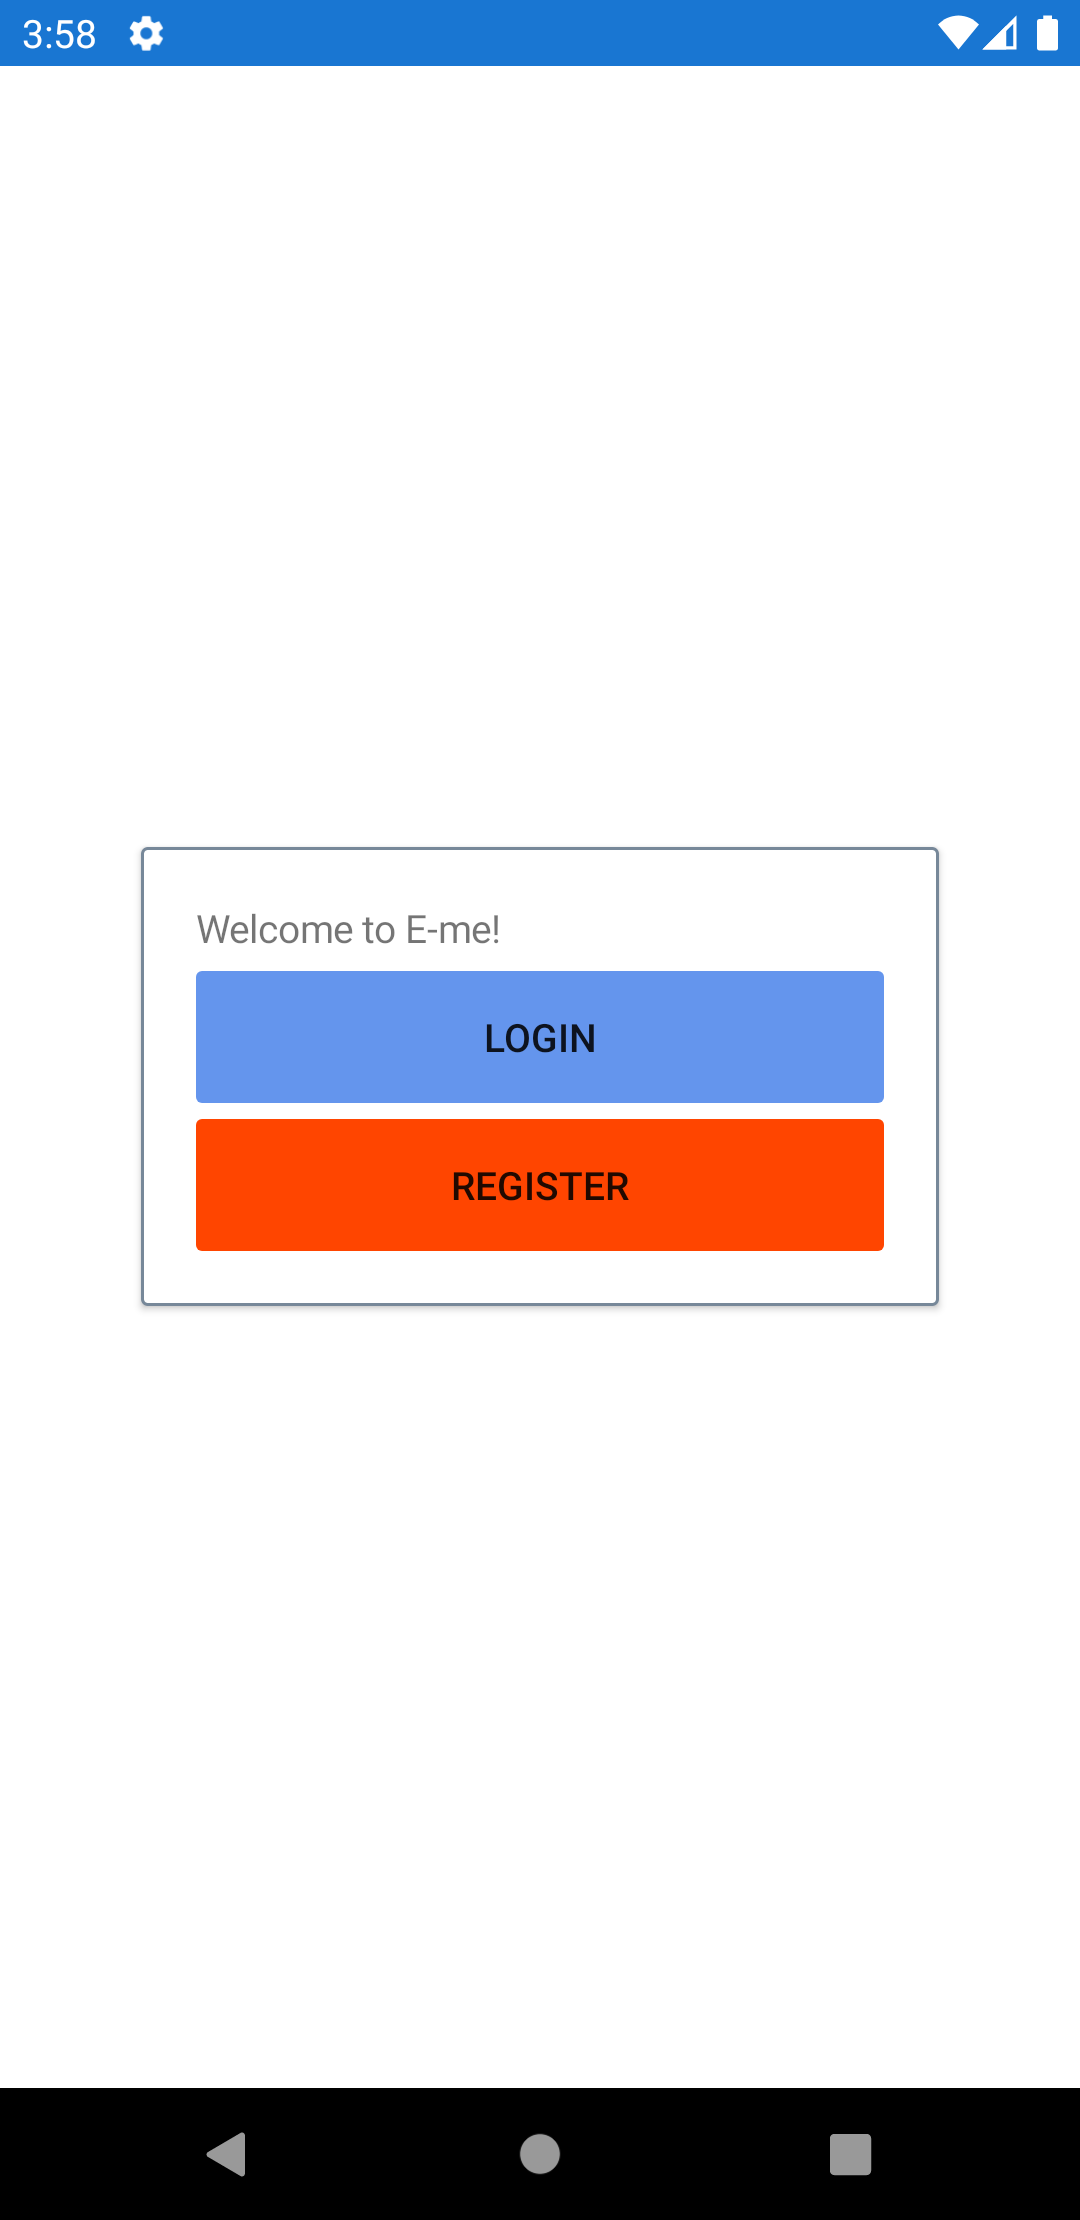
\includegraphics[scale=0.12]{main-page}				
			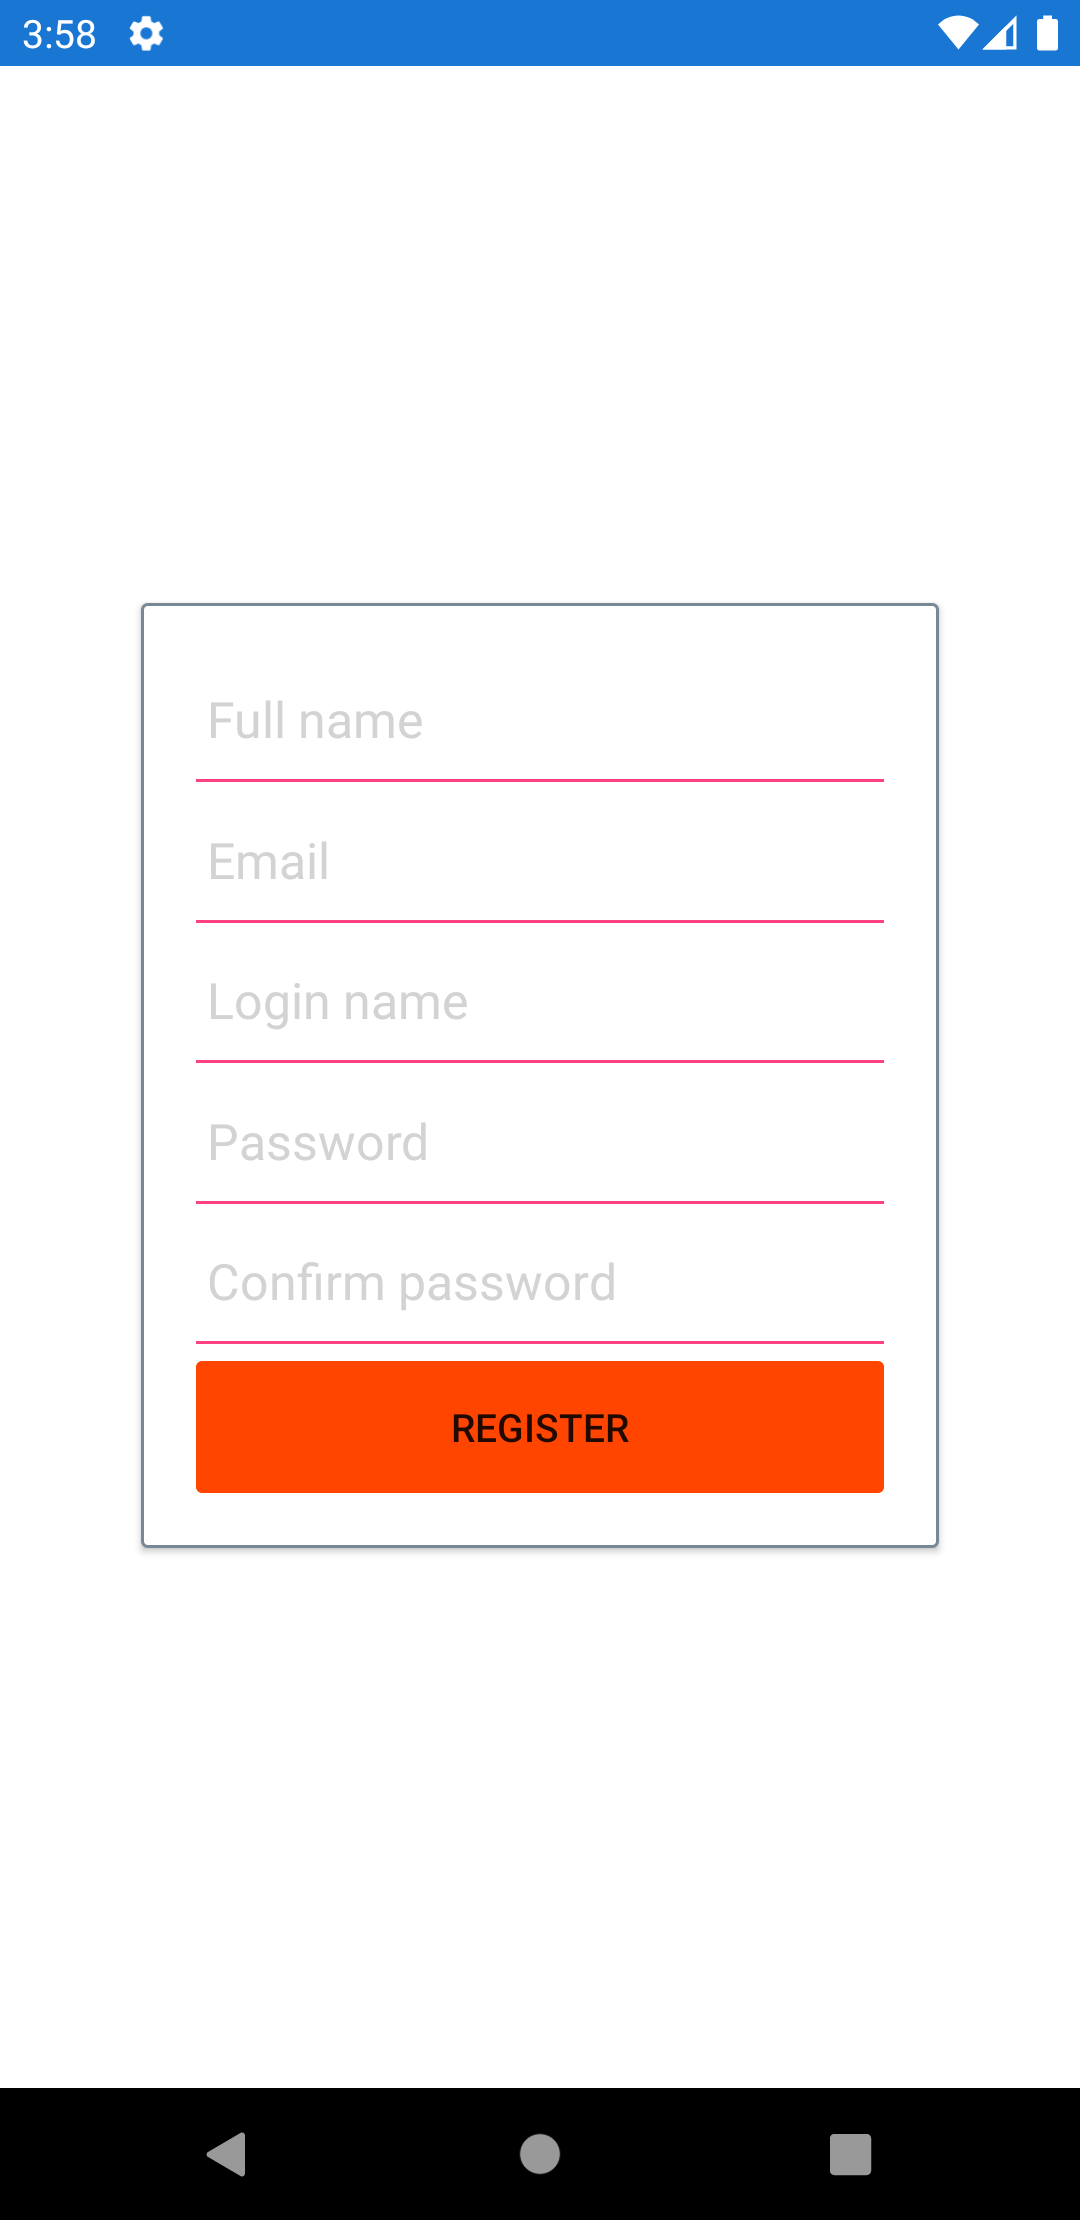
\includegraphics[scale=0.12]{register-page}			
			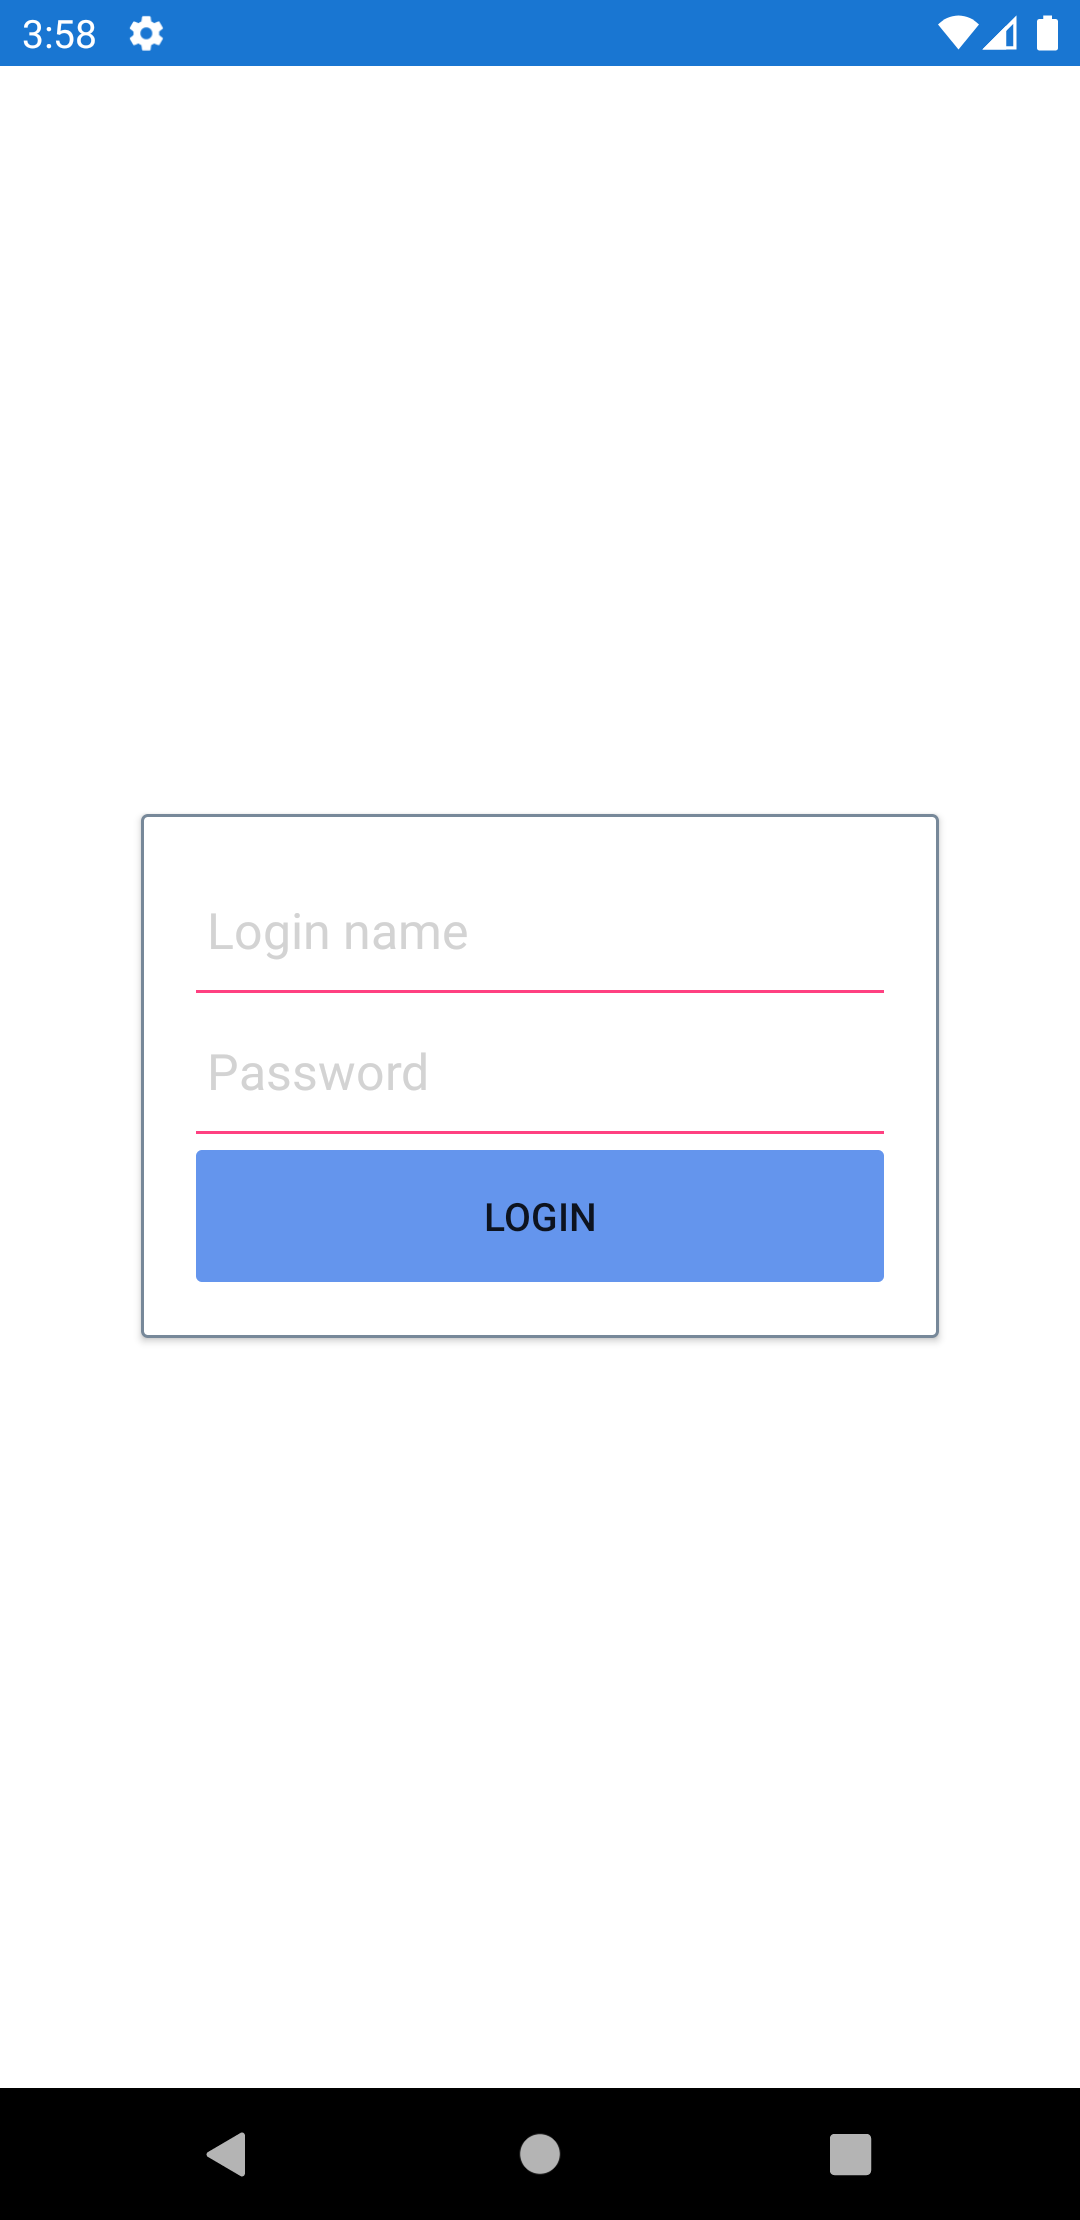
\includegraphics[scale=0.12]{login-page}				
			\caption{Introductory pages (Greeting, Registration, Login)}
		\end{figure}

	\section{My Documents}\label{documents}
	The My Documents page consists of two main parts: the list of documents and the "Scan QR code" button.
	The list of documents allows the user to visualize what types of documents they own.
	On each document two actions can be performed: Share and Remove.

		\begin{figure}[h]
			\centering
			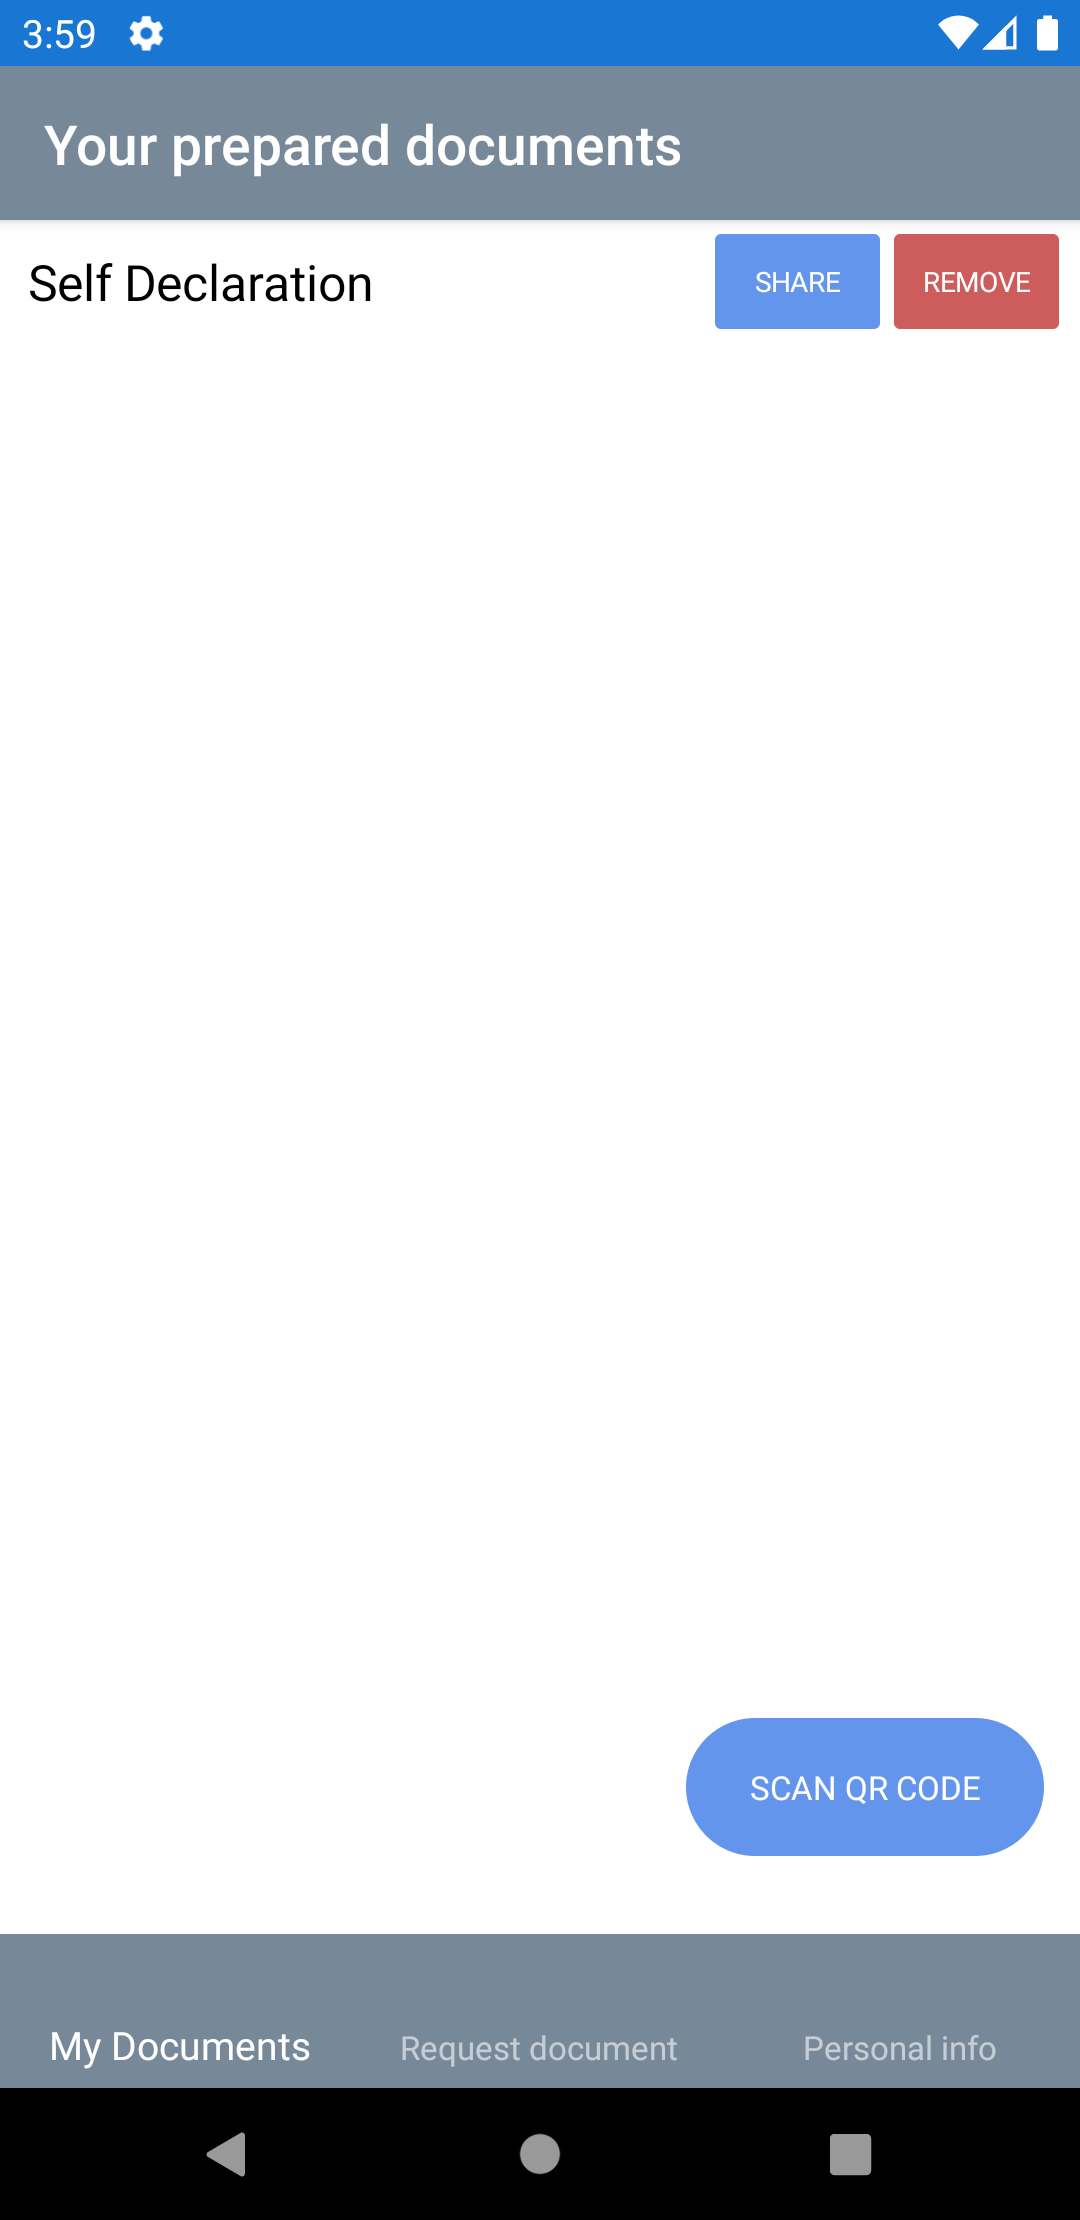
\includegraphics[scale=0.12]{documents-page}				
			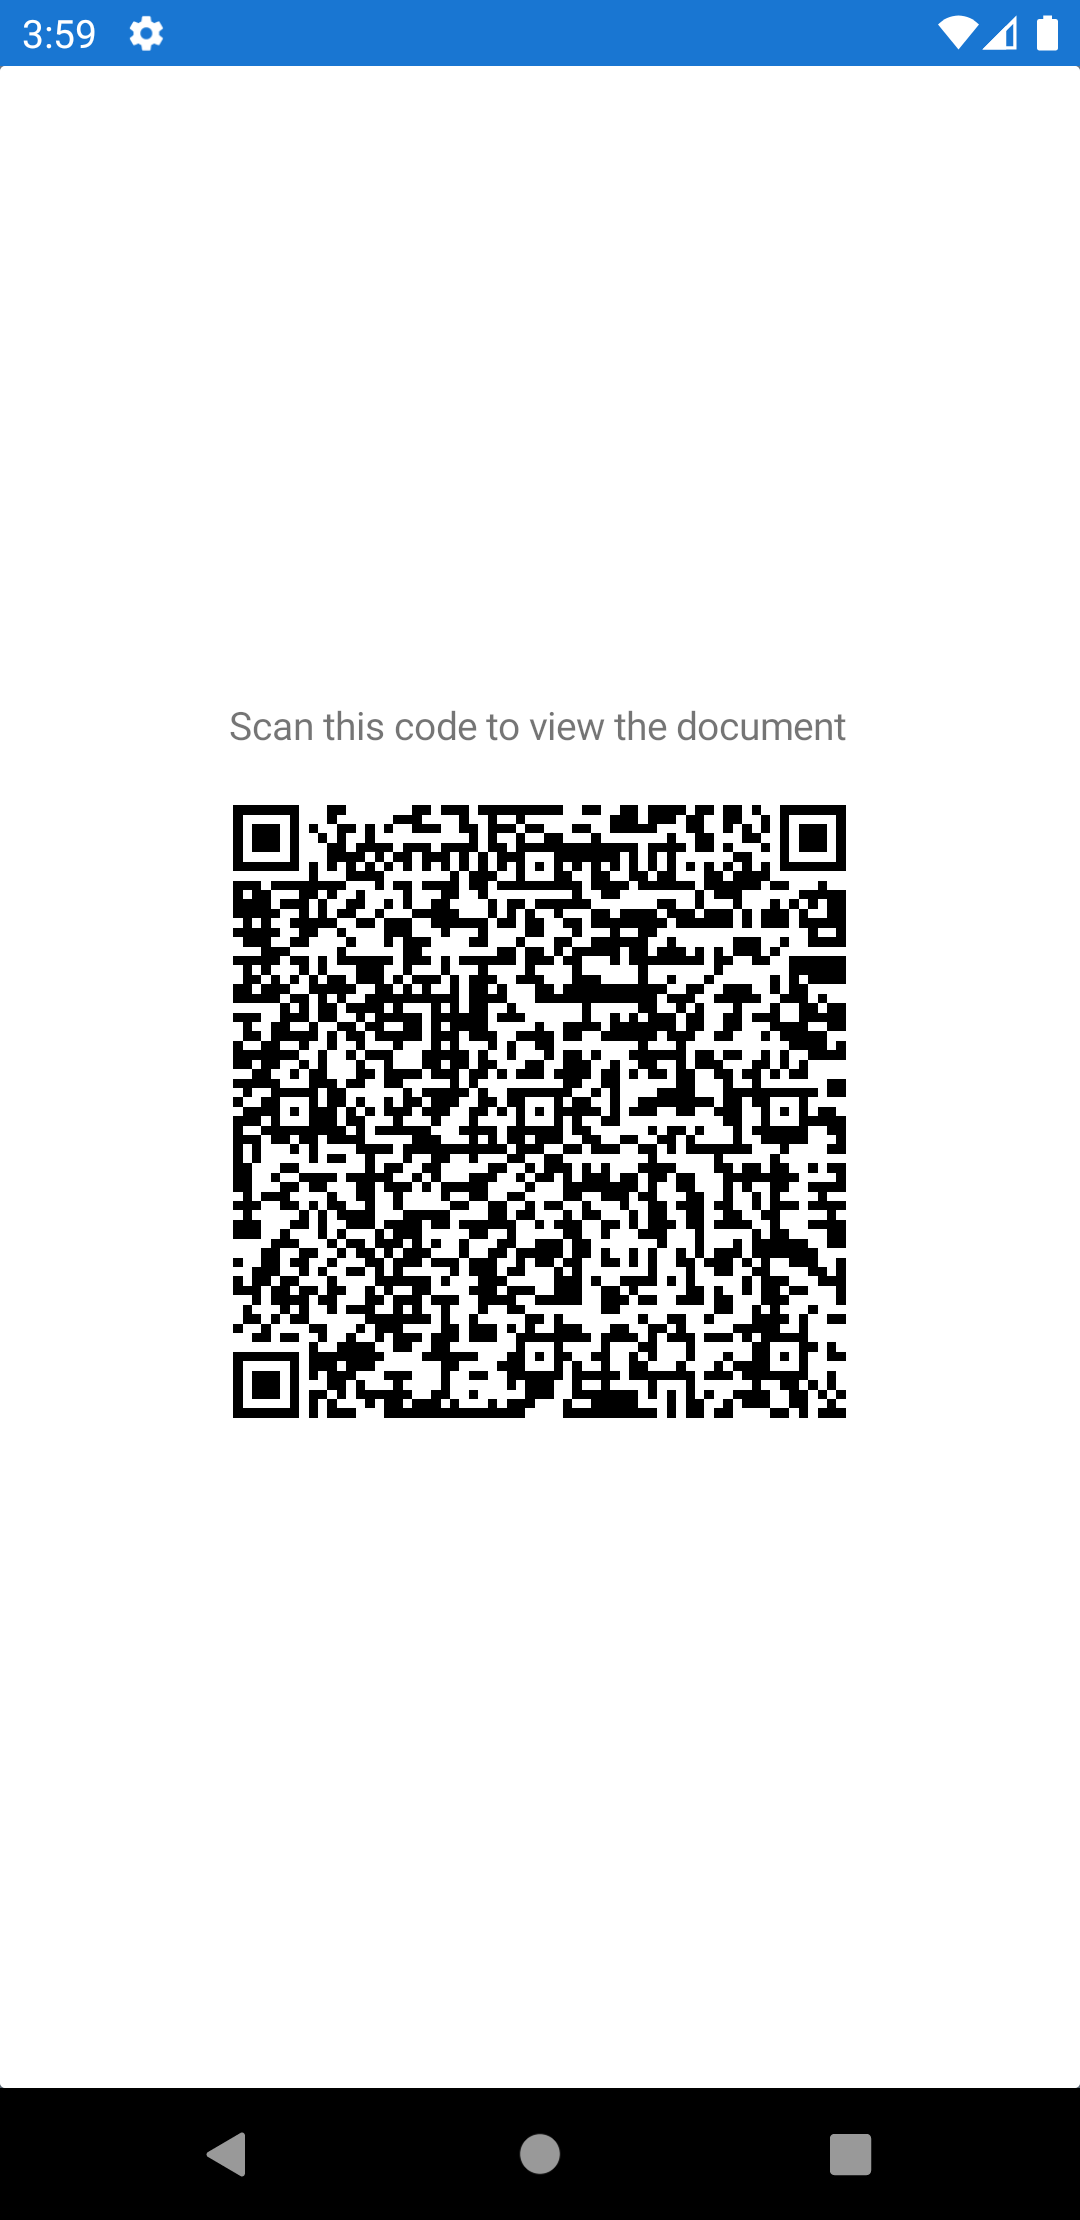
\includegraphics[scale=0.12]{share-document-page}
			\caption{Documents and Share Document pages}
		\end{figure}

		Tapping the Remove button irreversibly deletes the document from the list.
		After a successful removal the user is able to request a new document of the same type.
		If the document template was modified since
		the previous request or the user modified their personal information, the resulting document may be different than the previously deleted one.

		The Share button allows the user to safely transfer their selected document to a different device.
		Upon tapping the button, the application generates a unique code for the document which is then displayed on the screen via a QR code.

		The code can be read using the "Scan QR code" button. 
		Tapping this button will attempt to open the device's main camera in order to scan the code.
		If this feature is accessed for the first time, a prompt appears asking for the user's permission to use the camera.
		If the permission is granted, the application will open the camera app. 
		Upon successfully reading a QR code generated by E-me, the selected document will appear on the screen (see \hyperref[document]{Document Viewer}).

	\section{Requesting a Document}

	The Request Document page consists of a list of document types that can be acquired by the user.
	The list only contains types that are not yet owned by the corresponding user.
	If the user acquires one of these document types, it will disappear from the list (it will be listed on the \hyperref[documents]{My Documents} page instead).

	Combined with the \hyperref[documents]{My Documents} page, these two lists contain every document type that can be managed through the application. 
		\begin{figure}[h]
			\centering
			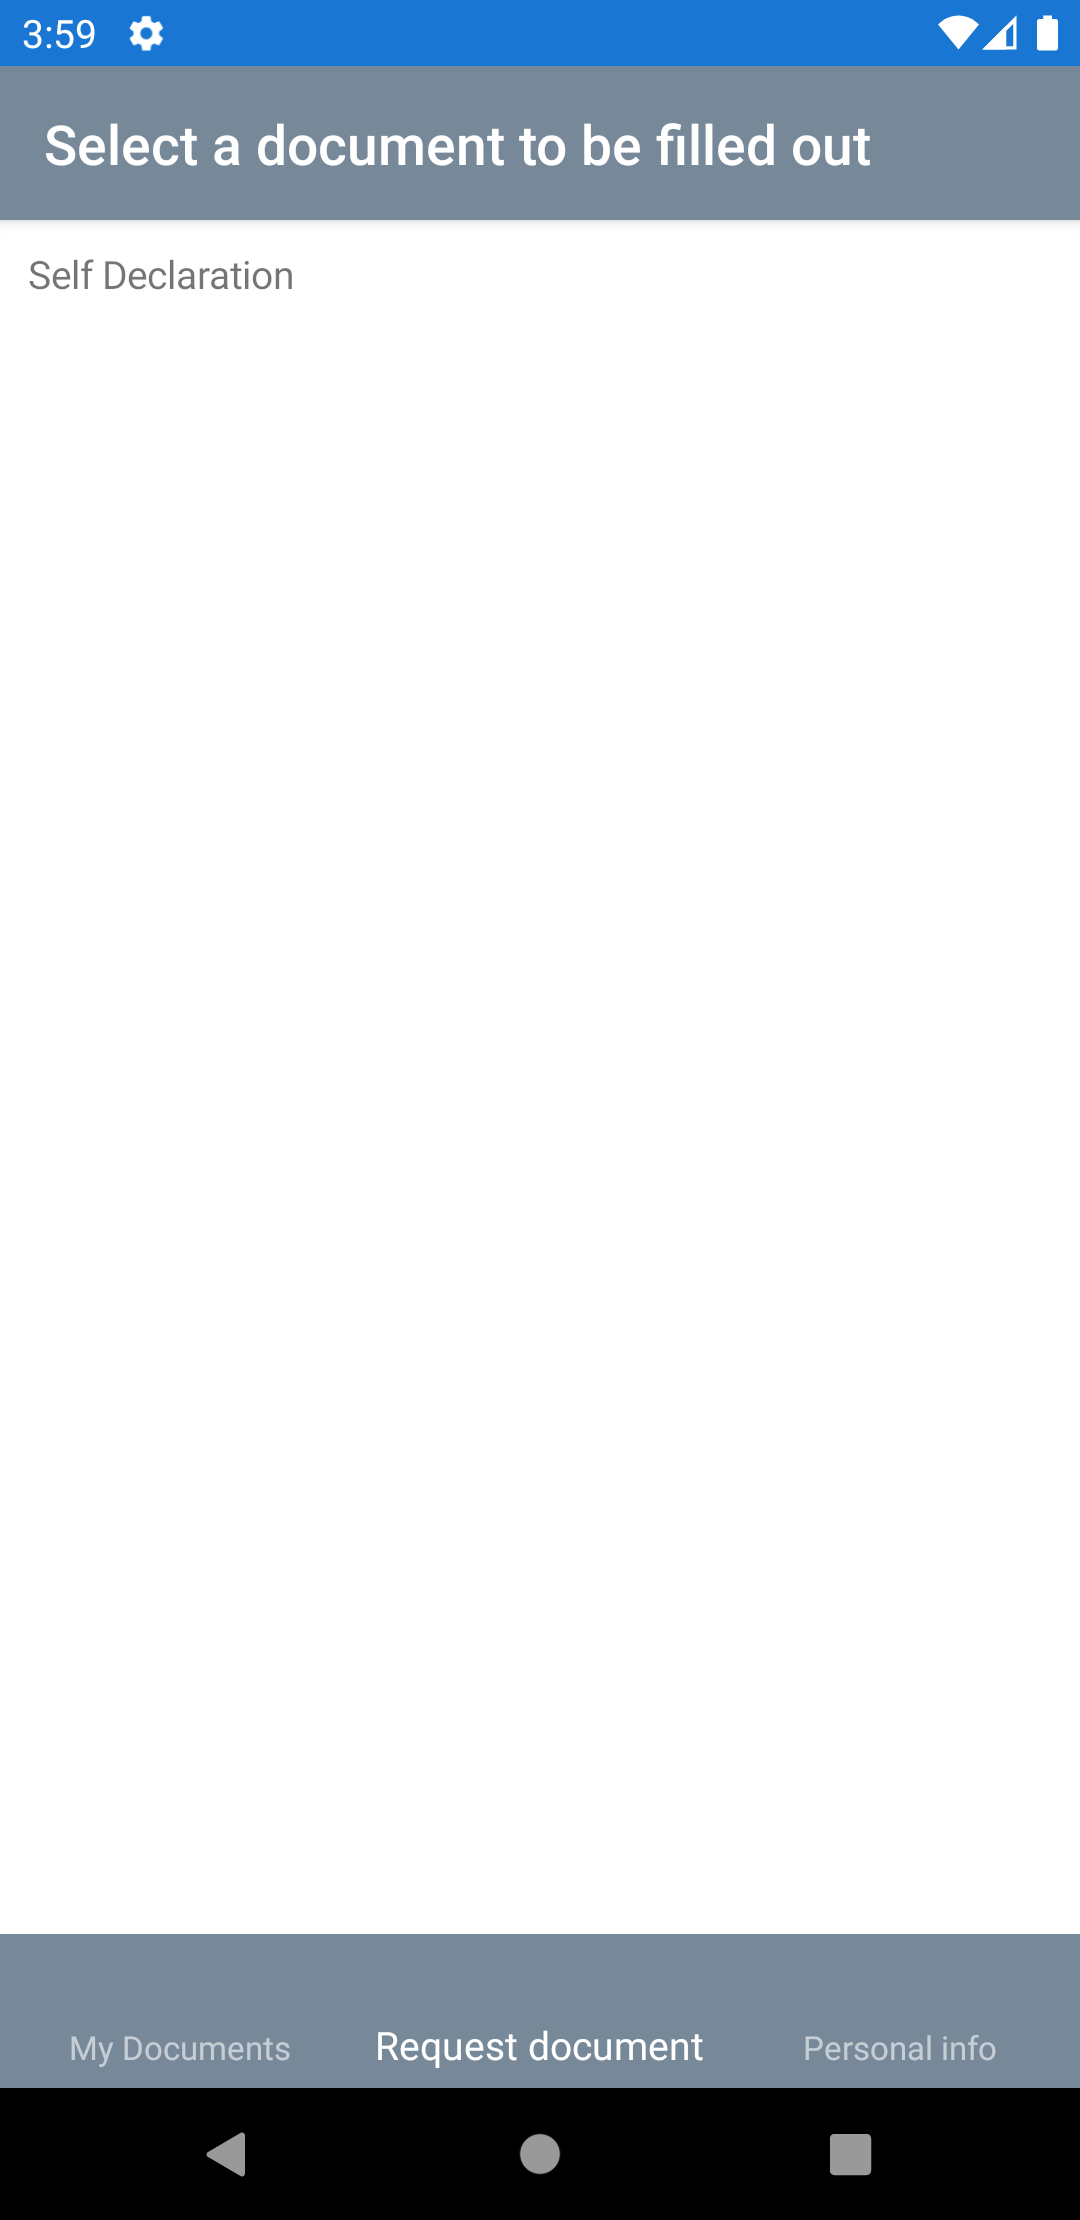
\includegraphics[scale=0.12]{request-document-page}				
			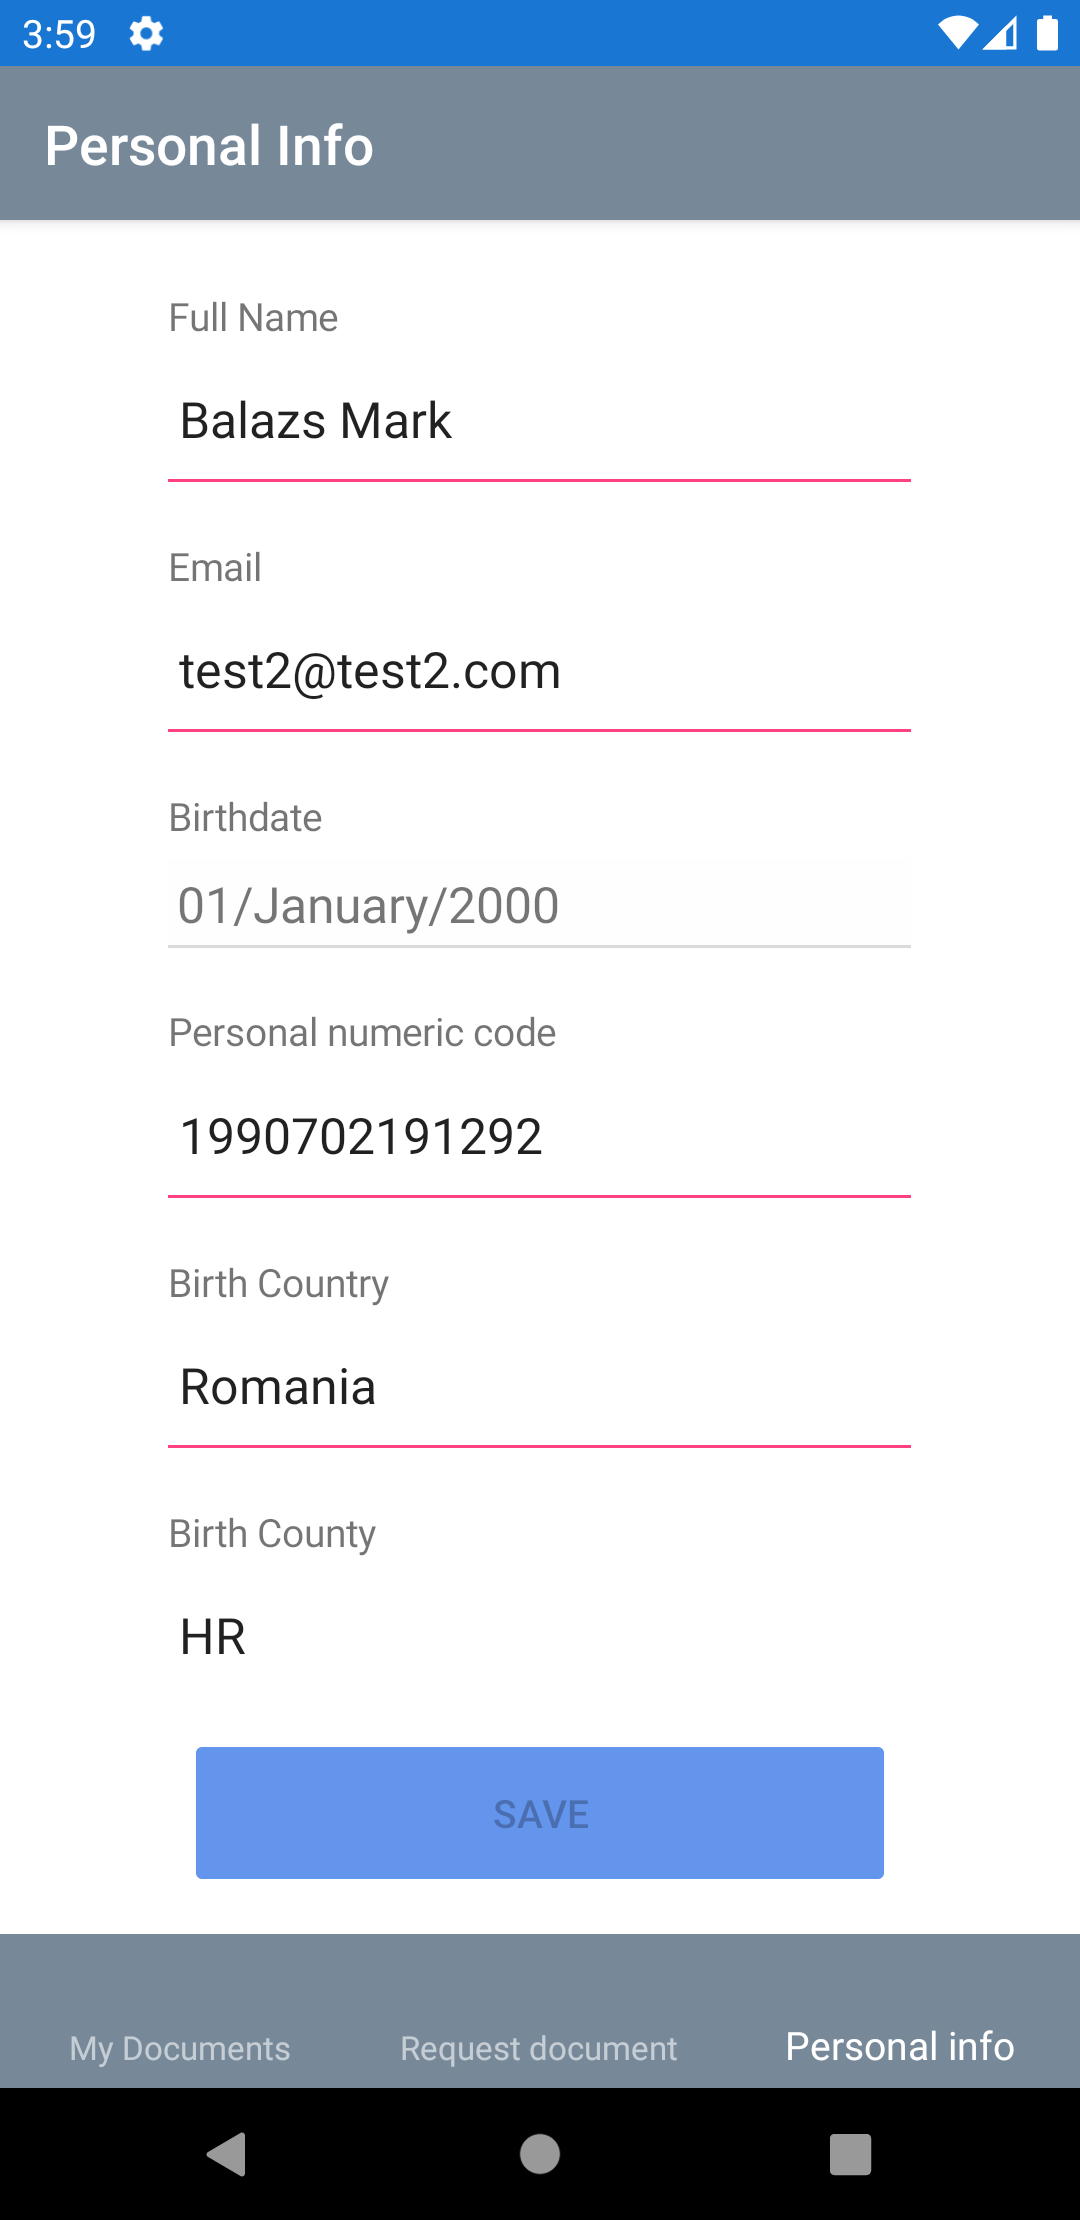
\includegraphics[scale=0.12]{personal-info-page}
			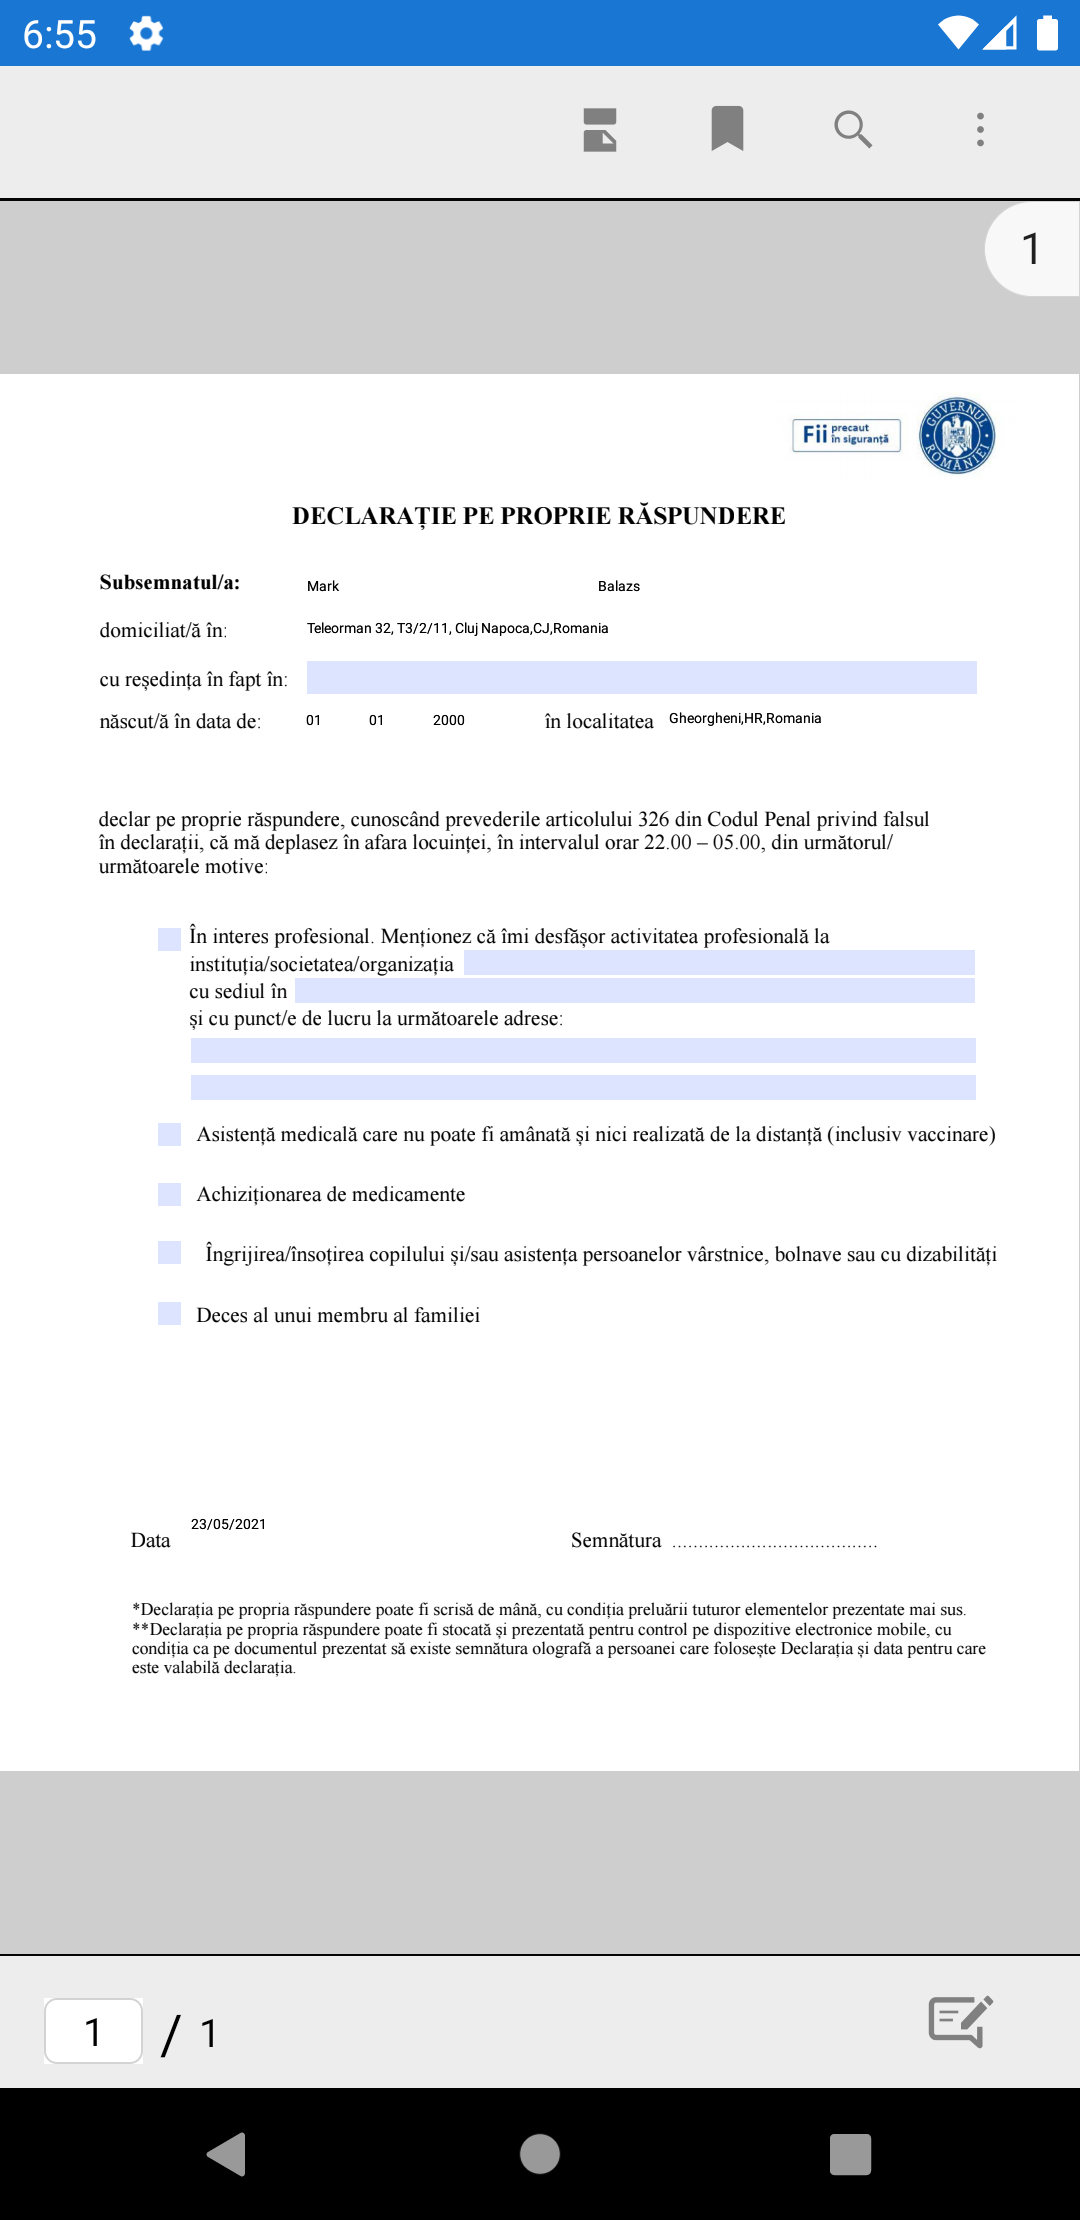
\includegraphics[scale=0.12]{document-page}
			\label{fig:document}
			\caption{Request Document, Personal Information and Document Viewer pages}
		\end{figure}

		The user can request a document by simply tapping on an item from the list. 
		The requested document will be generated and automatically displayed on the screen (see \hyperref[document]{Documents Page}).

	\section{Personal Information}

	This page contains several fields containing the personal details of the user. 
	Neither of these fields are required, however if no information is provided about the user, the application will not be able to automatically fill the requested documents.
	The information provided by the user on this page will be stored in an encrypted form.

	Upon requesting a document, E-me attempts to match the fields of the document with the information of the user and fill them out respectively.
	Fields that require information that is not provided by the user will be left blank and can be filled manually on the \hyperref[document]{Document Viewer}.

	\section{Document Viewer}\label{document}

	On this page a PDF Viewer can be seen which allows the user to inspect or even edit their documents.
	This viewer supports text searching, bookmarking, zooming, printing and/or saving a PDF to the local storage of the mobile device.
	The contents of the PDF are generated by the application, however if the document contains fields that could not be matched with any user data,
	the user is able to fill them out manually. This page can be closed by pressing the Back button.

	Figure \ref{fig:document} contains an example of a Romanian COVID-19 self-declaration.
	The document consists of multiple input types, including checkboxes, dates and text fields.
	The majority of these inputs refer to general information about the user (name, date of birth etc.) which can be filled out automatically by the application,
	 however some fields require time- or location-dependent data, which is not stored in E-me.
	 In this case, these fields are left blank so that the user is able to complete them manually.

%!TEX root = dolgozat.tex
%%%%%%%%%%%%%%%%%%%%%%%%%%%%%%%%%%%%%%%%%%%%%%%%%%%%%%%%%%%%%%%%%%%%%%%
\chapter{Technical details}\label{ch:IMPLEMENTATION}

\section{Architecture}

E-me follows a commonly used N-tier architecture with three main parts: data, application (backend) and presentation (frontend) layers.
Each of these tiers can be broken down into layers that are defined by their responsibilities within the application.
This tier-based architectural approach adds modularity to the application which results in a low cost of change when compared to a single-tier structure.

\begin{figure}[H]
	\centering
	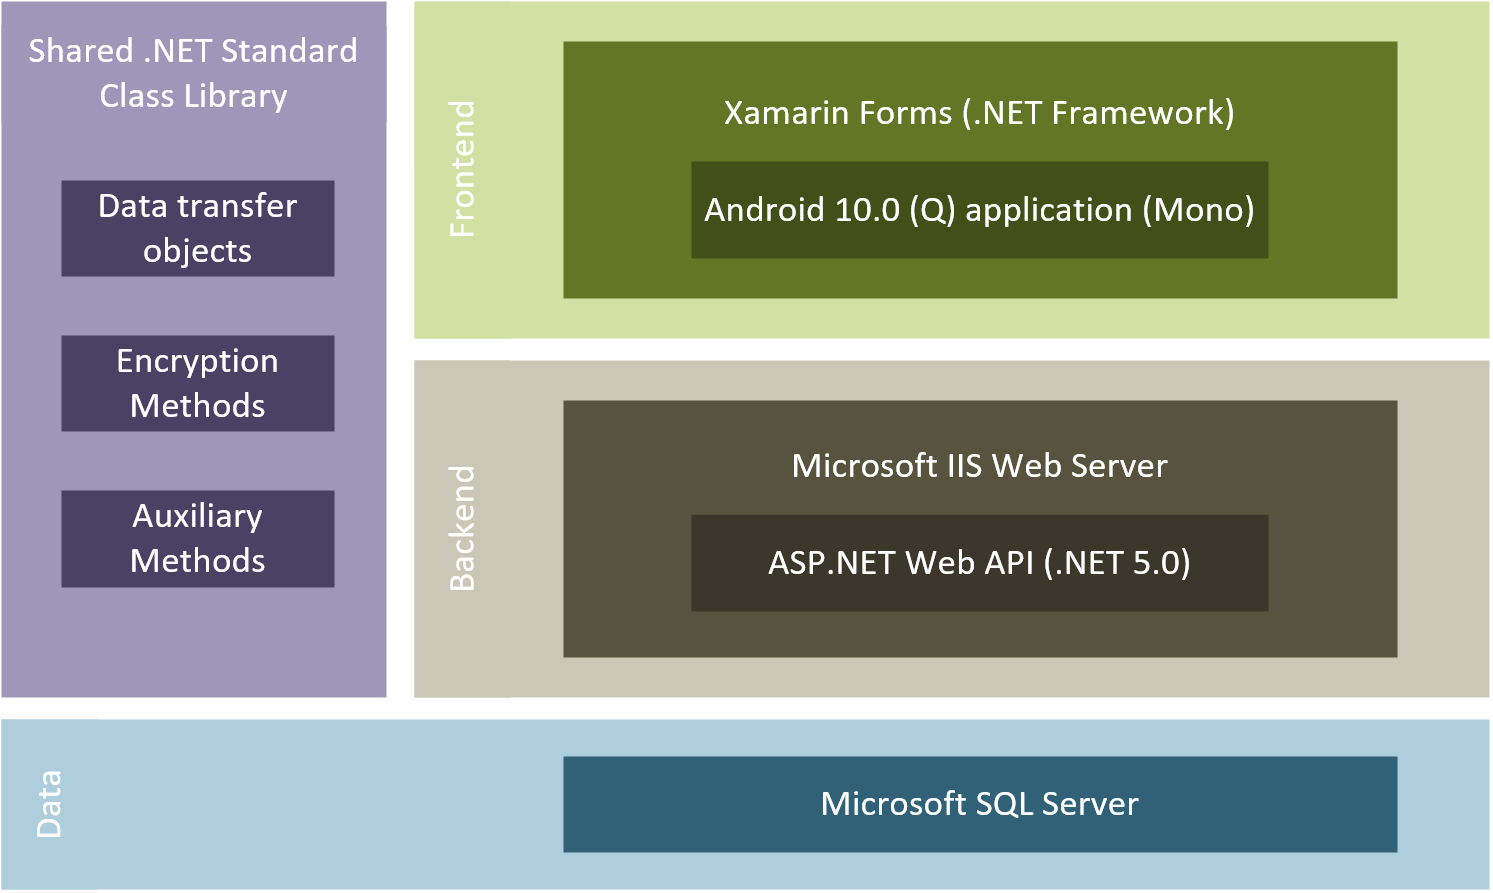
\includegraphics[scale=0.57]{general-architecture}
	\caption{General architecture}
\end{figure}

Along with the low cost of change, the independence of the layers allows for efficient future expansion of 
the application by means of multiple frontend platforms (ex. web applications, desktop applications), cloud storage/services and additional
Web API's that can easily be integrated into the existing application.
This, combined with the high compatibility of the .NET 5.0, provides a high level of scalability and maintainability for the application.

The application and presentation layers share a common class library that contains communication-related models and auxiliary methods.
This library allows both layers to benefit from the cross-platform nature of .NET 5.0, speeding up the process of development and
ensuring there are no discrepancies betweeen the layers in terms of encryption and communication.

\subsection{Application layer / Backend}

The architecture of the application layer has a similar design approach to the general architecture.
Consisting of 4 layers, the backend follows the single-responsibility principle in it's core.
Because of it's vertical structure, each layer is dependent on one single layer that is directly below it, providing a high level
of maintainability.

\begin{figure}[H]
	\centering
	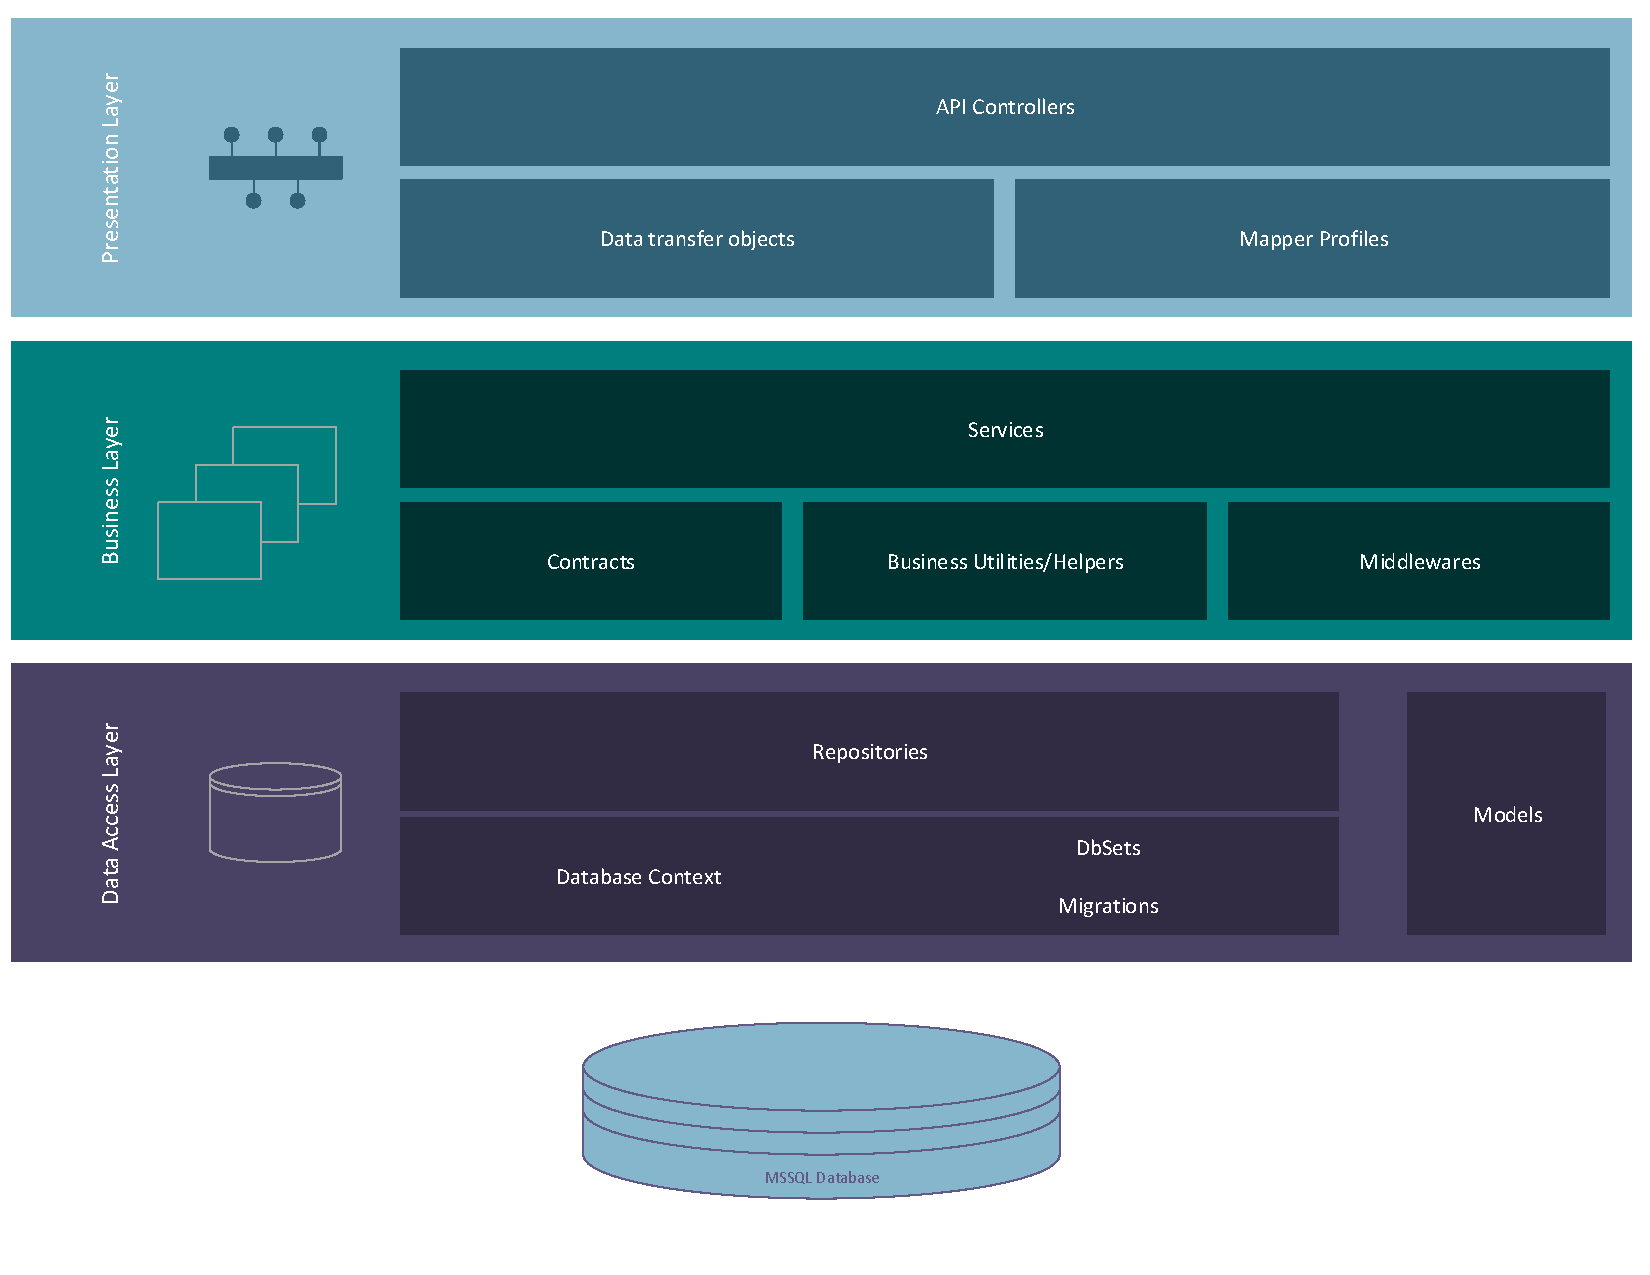
\includegraphics[scale=0.57]{backend-architecture}
	\caption{Backend architecture}
\end{figure}

Due to this abstract layout, each layer can independently be replaced or updated. 
This aspect enables the utilization of external and/or third-party services and components without damaging the integrity of the application.

The API structure of the presentation layer allows for a wide variety of applications or even services in which the backend can be used: desktop applications,
WPF, web servers and more. This characteristic has major role in preserving the flexibility of the application layer.

Another component being responsible for the independece and reusability of the backend is the Data Access Layer. 
The role of this layer is to provide the data requested by the Business Layer. 
By reason of abstraction, this layer is independent of the technology of the data source. 
This enables the utilization of a wide range of data sources, including relational (SQL) and non-relational (NoSQL) databases, cloud services and/or APIs.

\subsubsection{Entity relations in the application layer}


\begin{figure}[H]
	\centering
	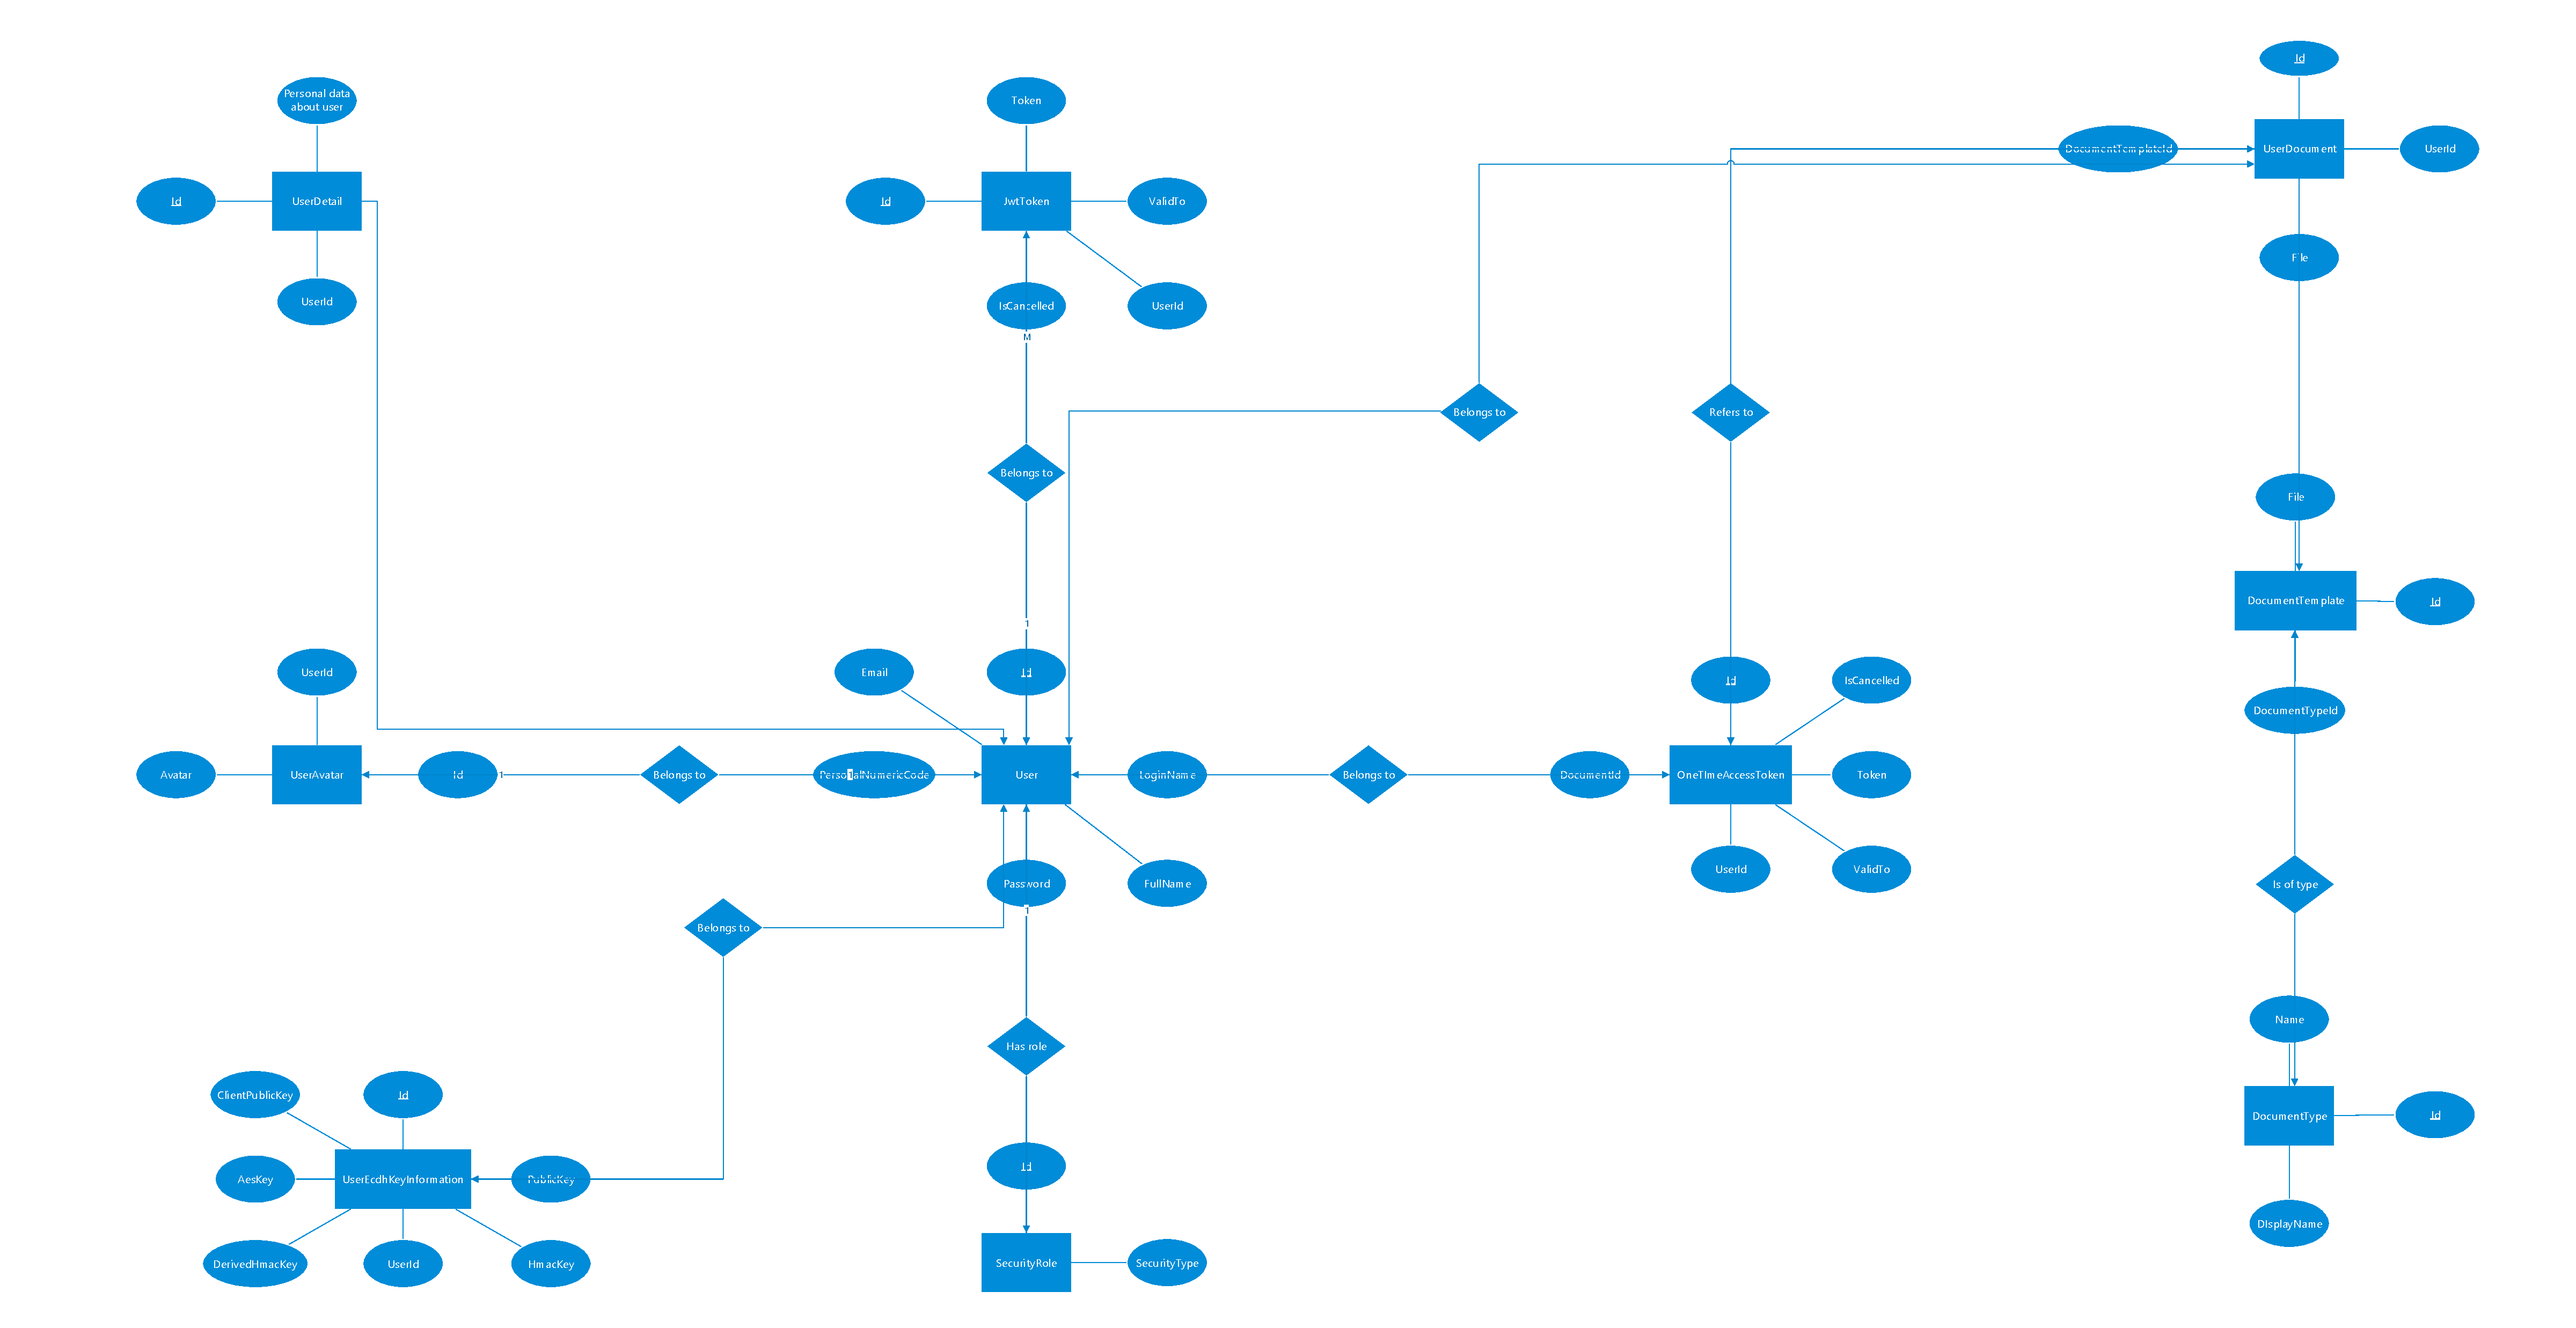
\includegraphics[scale=0.29]{entity-relationship-diagram}
	\caption{ER diagram}
\end{figure}

\subsection{Presentation layer / Frontend}

The frontend of the application consists of three major layers that separate the user interface from the business logic and the data sources.
This separation allows for easy horizontal expansion and quick feature development.

The Presentation or UI Layer contains the visuals of the application which are separated into independent pages, however it is also responsible for receiving
user events and connecting them with the underlying services.
Each page contains it's own event listeners and separate View Model that is responsible for making use of the Business Layer,
which has a similar structure and role to the backend's Business Layer: data processing and calculations.

The main components of the Data Layer are Data Stores.
These stores are functionally similar to the repositories found in the Backend of the application, although here the data is retrieved using the endpoints
of the backend.

\begin{figure}[H]
	\centering
	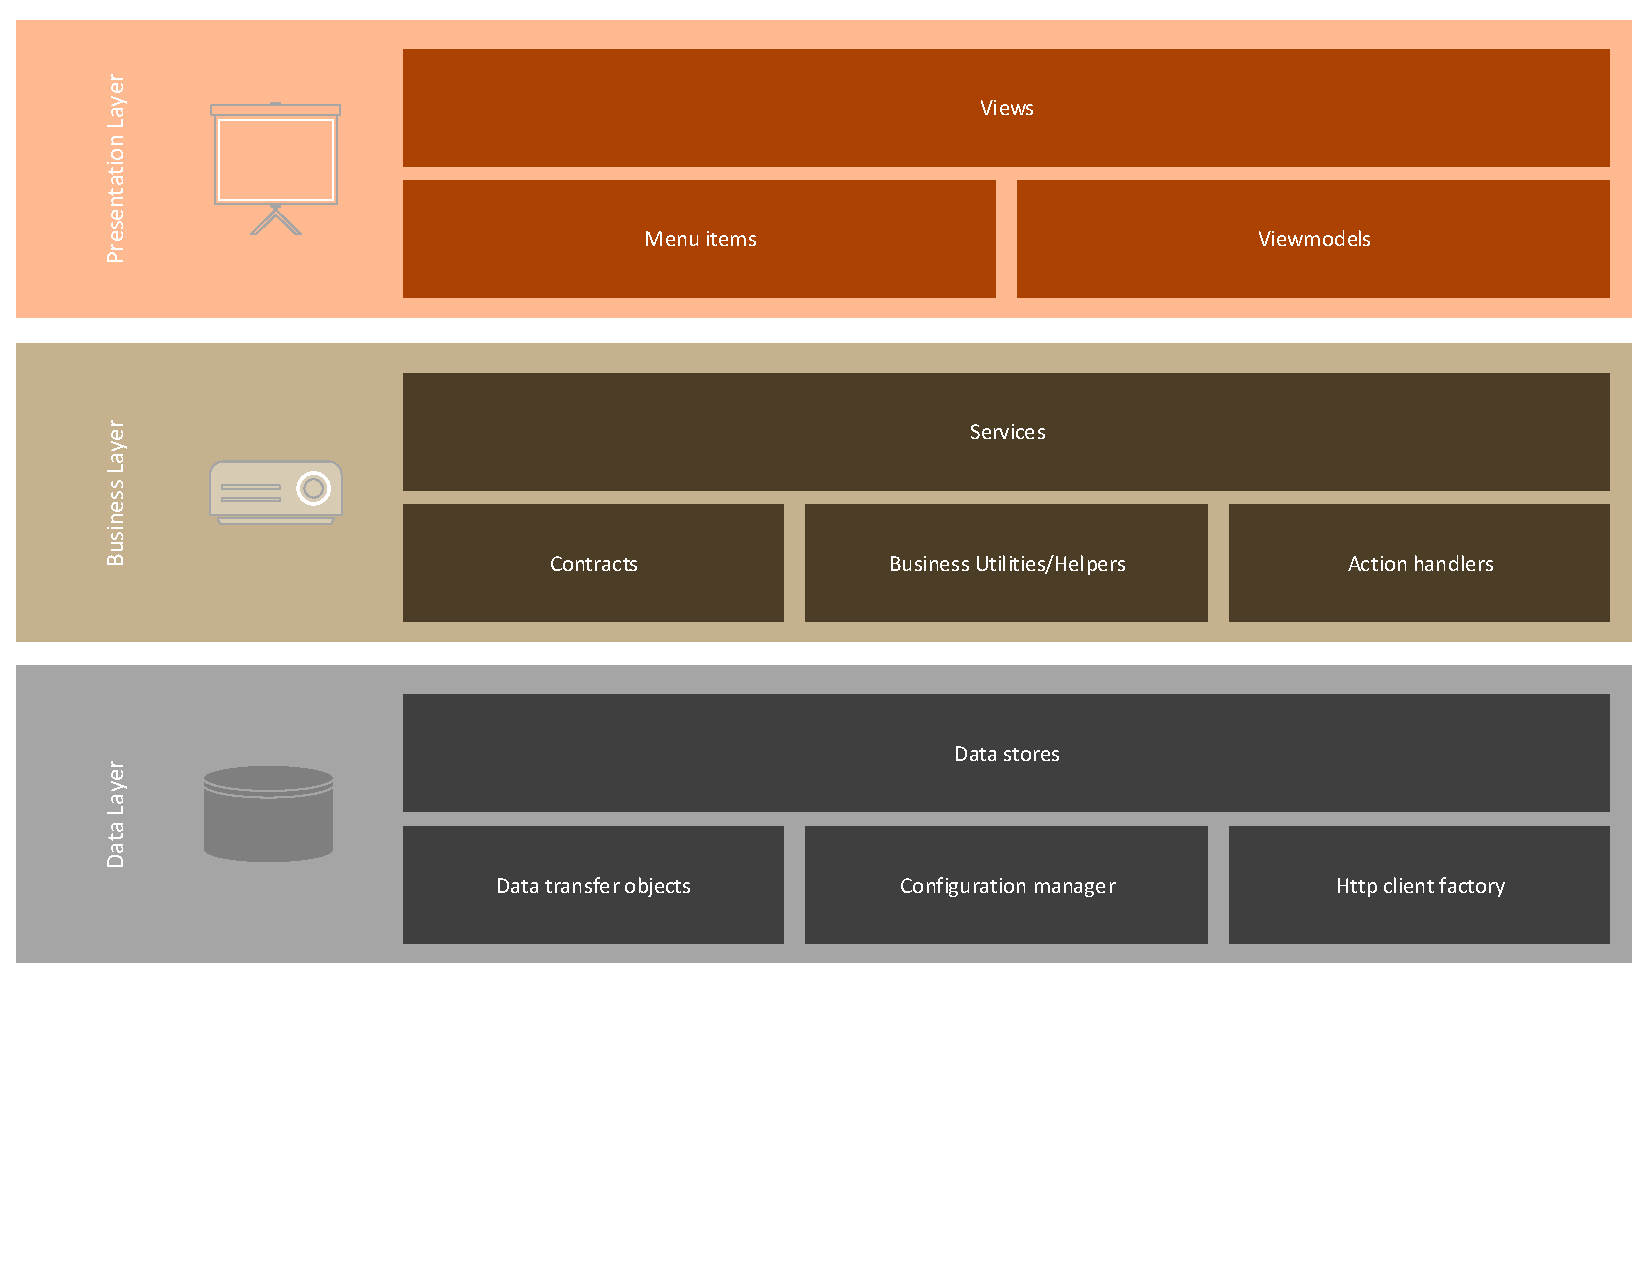
\includegraphics[scale=0.57]{frontend-architecture}
	\caption{Frontend architecture}
\end{figure}


%%%%%%%%%%%%%%%%%%%%%%%%%%%%%%%%%%%%%%%%%%%%%%%%%%%%%%%%%%%%%%%%%%%%%%%
\section{Technologies}

E-me makes great use of the cross-platform nature of .NET, meaning both the frontend and the backend of the application are implemented using the same
programming language: C\# 9.
The flexibility that is provided by the language and the wide variety of frameworks that make use of it allows for a cleaner codebase and a simpler
project structure when compared to a multilingual application design.

\subsection{Backend}

In terms of frameworks, the backend relies on .NET 5.0. Being the next major release of .NET Core following 3.1, this open-source cross-platform
software framework unifies a wide variety of frameworks .NET has to offer, including Windows Forms, ASP.NET Core, Azure and more.
This unification made the framework a perfect candidate for the backend of an application like E-me, since it can be used on a wide variety of
platforms and ensures long-term support.

E-me uses Internet Information Services (Microsoft IIS), which is an extensible web server software, as it's backend server.
It allows the application to communicate through HTTPS and provides it's separate development-time SSL certificate in order to secure the transport
layer. With the \emph{Development-time IIS support} feature, the web server allows \emph{hot reloading}, which speeds up the development and debugging
processes.

The main constituent of the backend itself is the ASP.NET Core web framework.
Using it's built-in IoC, this framework allows for a high level of abstraction in order to build well-structured enterprise level applications
using dependency injection.
This framework is responsible for registering and configuring any other dependencies that may appear in the application backend.

Alongside with ASP.NET Core, one of the main components of the backend is the Entity Framework Core, which is the base of the 
\emph{Data Access Layer}.
In terms of building and maintaining the data access layer, E-me uses the code-first approach through \emph{EF Migrations}.
This approach provides flexibility in case of a potential database change and/or creation, but more importantly it allows 
the entire structure of the entities to be managed based on the models and datasets present in the code.

Although the frameworks used by the layers of the application differ, these can have a shared codebase in the form
of a \emph{.NET Standard class library}, which can be used by both the backend and the frontend.

\begin{itemize}
	\item Backend
	\begin{itemize}
		\item .NET 5
		\item Entity Framework Core 5
		\begin{itemize}
			\item Code-first
			\item Microsoft SQL Server
			\item additional Data Encryption layer
		\end{itemize}
		\item NSwag
		\item Serilog
		\item AutoMapper
		\item Newtonsoft Json
		\item Windows CNG (Cryptographic Next Generation) API
	\end{itemize}
	\item Frontend
	\begin{itemize}
		\item Xamarin Forms
		\item Telerik UI for Xamarin
		\item Telerik Document Processing Core
		\item Syncfusion Xamarin PDF viewer
		\item GoogleVision API - BarcodeScanner XF implementation
	\end{itemize}
\end{itemize}

\section{Implementation}


\section{Security}
Here I describe the Diffie-Hellman key exchange and the used encryption techniques in more detail, 3-4 pages.

\begin{itemize}
	\item data-layer security
	\begin{itemize}
		\item using built-in EF Data Encryption with AES256
	\end{itemize}
	\item transport-layer security (TLS)
	\begin{itemize}
		\item https
		\item JWT auth and auth verification
		\item protected and unprotected endpoints
	\end{itemize}
	\item End-To-End encryption
	\begin{itemize}
		\item Elliptic Curve Diffie-Hellman key derivation - open-source implementation
		\item encryption of documents
		\item hash-based message authentication (HMAC)
	\end{itemize}
\end{itemize}

%!TEX root = dolgozat.tex
%%%%%%%%%%%%%%%%%%%%%%%%%%%%%%%%%%%%%%%%%%%%%%%%%%%%%%%%%%%%%%%%%%%%%%%
\chapter{Results and evaluation}\label{ch:elemzes}
\begin{summary}
	In this chapter I describe decisions I made, difficulties I faced during development and the quality of my code.
\end{summary}


\section{Metrics}
In this section I will evaluate some of the algorithms used in the application, test coverage, code analysis. 4 pages

\begin{figure}[H]
	\centering
	\definecolor{mycolor1}{rgb}{0.00000,0.44700,0.74100}%
\definecolor{mycolor2}{rgb}{0.85000,0.32500,0.09800}%
\definecolor{mycolor3}{rgb}{0.92900,0.69400,0.12500}%
%
\begin{tikzpicture}

\begin{axis}[%
width=5.520833in,
height=3.065625in,
at={(1in,2in)},
scale only axis,
xmin=0,
xmax=1600000,
xlabel={File size (Kilobytes)},
ymin=0,
ymax=200000,
ylabel={Execution time (ticks)},
axis x line*=bottom,
axis y line*=left,
legend style={legend cell align=left,align=left,draw=white!5!black}
]
\addplot[const plot,color=mycolor1,line width=0.8pt,mark size=1.0pt,mark=.,mark options={solid}] plot table[row sep=crcr] {%
15360 2018 \\
20480 1357 \\
25600 1591 \\
30720 2498 \\
35840 2639 \\
40960 3029 \\
46080 2787 \\
51200 3145 \\
56320 3472 \\
61440 3755 \\
66560 3638 \\
71680 3564 \\
76800 4115 \\
87040 4307 \\
92160 4963 \\
102400 4870 \\
107520 4779 \\
112640 6593 \\
117760 5766 \\
122880 7444 \\
128000 5969 \\
133120 6374 \\
138240 6624 \\
143360 8358 \\
148480 8198 \\
158720 7587 \\
163840 7985 \\
168960 10085 \\
174080 10472 \\
179200 11641 \\
184320 8960 \\
189440 11437 \\
194560 9957 \\
199680 13331 \\
204800 11080 \\
209920 10291 \\
215040 11825 \\
220160 10043 \\
225280 10438 \\
230400 11665 \\
235520 14040 \\
240640 11276 \\
245760 11293 \\
250880 11471 \\
256000 13528 \\
261120 11847 \\
266240 12915 \\
271360 16094 \\
276480 16106 \\
281600 15251 \\
291840 17883 \\
296960 18958 \\
302080 16604 \\
307200 17276 \\
312320 15151 \\
317440 17860 \\
322560 16281 \\
327680 19143 \\
332800 18058 \\
337920 15081 \\
343040 16324 \\
348160 16002 \\
353280 15300 \\
358400 18342 \\
363520 21446 \\
368640 17409 \\
373760 20767 \\
378880 27074 \\
384000 22992 \\
389120 18067 \\
394240 21159 \\
399360 19668 \\
404480 24201 \\
409600 19469 \\
414720 20307 \\
419840 23584 \\
424960 19998 \\
430080 20433 \\
435200 22381 \\
440320 22013 \\
445440 27650 \\
450560 22065 \\
455680 26858 \\
460800 20586 \\
465920 20583 \\
471040 22196 \\
476160 24696 \\
481280 23727 \\
486400 24082 \\
491520 21874 \\
496640 25353 \\
501760 22471 \\
506880 25445 \\
512000 26921 \\
517120 26333 \\
522240 30998 \\
527360 27583 \\
532480 24332 \\
537600 24176 \\
542720 24503 \\
568320 25723 \\
573440 27844 \\
578560 25805 \\
583680 30270 \\
588800 30891 \\
593920 27697 \\
599040 35783 \\
609280 31749 \\
614400 27735 \\
619520 27468 \\
624640 30130 \\
629760 32453 \\
634880 28522 \\
645120 29331 \\
650240 37720 \\
655360 37408 \\
660480 33583 \\
665600 33526 \\
670720 30320 \\
675840 35929 \\
680960 30644 \\
686080 35664 \\
691200 39906 \\
696320 31537 \\
701440 36834 \\
706560 40858 \\
711680 39346 \\
716800 39904 \\
721920 35975 \\
727040 31927 \\
732160 33434 \\
737280 41742 \\
742400 50994 \\
747520 46849 \\
752640 46972 \\
757760 43353 \\
768000 38407 \\
773120 40474 \\
778240 61574 \\
783360 48102 \\
788480 39538 \\
793600 39543 \\
798720 46258 \\
803840 39234 \\
808960 37406 \\
814080 40960 \\
819200 40752 \\
824320 39588 \\
829440 37850 \\
834560 42111 \\
839680 38641 \\
844800 44358 \\
849920 38521 \\
855040 44214 \\
860160 41120 \\
865280 40333 \\
870400 43604 \\
875520 43414 \\
880640 39986 \\
885760 41903 \\
890880 39896 \\
896000 46141 \\
901120 47058 \\
906240 45466 \\
911360 42942 \\
916480 47424 \\
921600 42783 \\
926720 48551 \\
931840 46662 \\
936960 48113 \\
942080 44889 \\
947200 46631 \\
952320 43063 \\
957440 49236 \\
962560 57885 \\
967680 46493 \\
972800 47425 \\
977920 47431 \\
983040 45642 \\
988160 45991 \\
993280 46480 \\
998400 48660 \\
1003520 46578 \\
1008640 48315 \\
1013760 46113 \\
1018880 53515 \\
1034240 49470 \\
1039360 51201 \\
1044480 51270 \\
1049600 49855 \\
1054720 53067 \\
1059840 52876 \\
1064960 48322 \\
1070080 49762 \\
1085440 59417 \\
1090560 50088 \\
1095680 49403 \\
1100800 57204 \\
1105920 51849 \\
1111040 51313 \\
1116160 53839 \\
1121280 50976 \\
1126400 52408 \\
1131520 52156 \\
1136640 59547 \\
1141760 54125 \\
1146880 64925 \\
1167360 58298 \\
1172480 52506 \\
1177600 53479 \\
1182720 60605 \\
1192960 54752 \\
1213440 56962 \\
1218560 59471 \\
1223680 59170 \\
1228800 58236 \\
1233920 56605 \\
1239040 71838 \\
1244160 60592 \\
1249280 60771 \\
1254400 67252 \\
1259520 76426 \\
1264640 76324 \\
1269760 78831 \\
1274880 62016 \\
1280000 57834 \\
1285120 63712 \\
1290240 61992 \\
1295360 78662 \\
1300480 66388 \\
1305600 87359 \\
1310720 83936 \\
1315840 88816 \\
1320960 63116 \\
1326080 63032 \\
1331200 61154 \\
1336320 67428 \\
1341440 86638 \\
1346560 69867 \\
1351680 91105 \\
1356800 91611 \\
1361920 89949 \\
1367040 62075 \\
1372160 69961 \\
1377280 61957 \\
1382400 66898 \\
1387520 85745 \\
1392640 62746 \\
1397760 80879 \\
1402880 81967 \\
1408000 81637 \\
1413120 63158 \\
1418240 67912 \\
1423360 69089 \\
1428480 73945 \\
1433600 87884 \\
1438720 68270 \\
1443840 94084 \\
1448960 93958 \\
1454080 89500 \\
1459200 66778 \\
1464320 69808 \\
1469440 67965 \\
1474560 71877 \\
1479680 89308 \\
1484800 71806 \\
1489920 96449 \\
1495040 95678 \\
1500160 94474 \\
1505280 72222 \\
1510400 74279 \\
1515520 70375 \\
1520640 78419 \\
1525760 94683 \\
1530880 74933 \\
1536000 93221 \\
1541120 95945 \\
};
\addlegendentry{Encryption};

\addplot[const plot,color=mycolor2,line width=0.8pt,mark size=1.0pt,mark=.,mark options={solid}] plot table[row sep=crcr] {%
15360 3068 \\
20480 2364 \\
25600 2902 \\
30720 2775 \\
35840 3245 \\
40960 4389 \\
46080 3856 \\
51200 4475 \\
56320 5258 \\
61440 5252 \\
71680 5429 \\
76800 5206 \\
81920 6130 \\
87040 7085 \\
92160 6458 \\
97280 7929 \\
107520 6714 \\
112640 10491 \\
117760 7716 \\
122880 9526 \\
128000 8803 \\
133120 8981 \\
138240 8815 \\
143360 9982 \\
148480 9949 \\
158720 10162 \\
163840 15312 \\
168960 12418 \\
174080 13302 \\
179200 13815 \\
184320 12227 \\
189440 14479 \\
194560 14772 \\
199680 15387 \\
204800 14207 \\
209920 21999 \\
215040 14018 \\
220160 13883 \\
225280 14950 \\
230400 17365 \\
235520 14132 \\
240640 14975 \\
245760 15144 \\
250880 15739 \\
256000 18159 \\
261120 19694 \\
266240 21478 \\
271360 17662 \\
276480 19315 \\
281600 18429 \\
286720 29777 \\
291840 17618 \\
296960 26890 \\
302080 23268 \\
307200 22142 \\
312320 23991 \\
317440 22699 \\
322560 23238 \\
327680 20657 \\
332800 22368 \\
337920 21347 \\
343040 23482 \\
348160 23502 \\
353280 21899 \\
358400 23296 \\
363520 23508 \\
368640 28314 \\
373760 23730 \\
378880 23163 \\
384000 28347 \\
389120 28598 \\
394240 24683 \\
399360 26383 \\
404480 30613 \\
409600 32140 \\
414720 28858 \\
419840 26843 \\
424960 27782 \\
430080 35721 \\
435200 28329 \\
440320 27330 \\
445440 32880 \\
450560 34461 \\
455680 32056 \\
460800 28949 \\
465920 29774 \\
471040 31987 \\
476160 30263 \\
481280 31425 \\
486400 30659 \\
491520 42405 \\
496640 31554 \\
501760 29907 \\
506880 33554 \\
512000 38345 \\
522240 34166 \\
527360 39612 \\
532480 36935 \\
537600 40919 \\
542720 36329 \\
547840 39955 \\
573440 34750 \\
578560 35503 \\
583680 40421 \\
588800 41380 \\
593920 37596 \\
599040 38545 \\
609280 42491 \\
614400 38796 \\
619520 37593 \\
624640 38921 \\
629760 44826 \\
634880 41472 \\
640000 39994 \\
645120 42347 \\
650240 41878 \\
655360 42548 \\
660480 46473 \\
665600 42915 \\
670720 45103 \\
675840 48051 \\
680960 42493 \\
686080 46169 \\
691200 47090 \\
696320 44076 \\
701440 43483 \\
706560 53429 \\
711680 51044 \\
721920 44768 \\
727040 43595 \\
732160 48413 \\
737280 44104 \\
742400 53609 \\
747520 57877 \\
752640 59118 \\
757760 58808 \\
768000 51460 \\
773120 48340 \\
778240 56085 \\
783360 57179 \\
788480 55971 \\
793600 49282 \\
803840 51573 \\
808960 54472 \\
814080 58405 \\
819200 51957 \\
824320 50115 \\
829440 53235 \\
834560 63102 \\
839680 50800 \\
844800 49872 \\
849920 55402 \\
855040 59735 \\
860160 56138 \\
865280 51480 \\
870400 56493 \\
875520 61505 \\
880640 52364 \\
885760 57642 \\
890880 61837 \\
896000 59193 \\
901120 56479 \\
906240 56117 \\
911360 56929 \\
916480 64725 \\
921600 57452 \\
926720 59476 \\
931840 58158 \\
936960 68887 \\
942080 59955 \\
947200 62406 \\
952320 66730 \\
957440 66414 \\
962560 57054 \\
967680 64871 \\
972800 64207 \\
977920 67162 \\
983040 61336 \\
988160 62373 \\
993280 62882 \\
998400 71250 \\
1003520 64169 \\
1008640 61717 \\
1013760 76290 \\
1018880 72096 \\
1034240 67002 \\
1039360 76511 \\
1044480 67124 \\
1049600 65937 \\
1054720 67993 \\
1059840 66257 \\
1064960 77925 \\
1070080 72437 \\
1075200 75919 \\
1080320 85705 \\
1085440 82641 \\
1090560 65301 \\
1095680 69996 \\
1100800 70172 \\
1105920 69133 \\
1111040 68685 \\
1116160 66118 \\
1121280 85934 \\
1126400 69846 \\
1131520 66778 \\
1136640 98608 \\
1141760 73523 \\
1146880 79052 \\
1152000 89318 \\
1157120 91090 \\
1162240 90516 \\
1167360 73422 \\
1172480 71586 \\
1177600 75257 \\
1182720 71008 \\
1187840 74084 \\
1192960 77559 \\
1203200 93028 \\
1208320 96833 \\
1213440 81241 \\
1218560 75969 \\
1223680 76858 \\
1228800 80982 \\
1233920 82308 \\
1239040 95678 \\
1244160 93605 \\
1249280 79229 \\
1254400 80130 \\
1259520 94947 \\
1264640 95030 \\
1274880 83502 \\
1280000 77134 \\
1285120 86858 \\
1290240 84628 \\
1295360 80924 \\
1300480 81470 \\
1305600 97093 \\
1320960 85634 \\
1326080 83026 \\
1331200 84031 \\
1336320 82088 \\
1341440 81379 \\
1346560 87653 \\
1367040 85559 \\
1372160 82211 \\
1377280 90993 \\
1382400 84255 \\
1387520 88830 \\
1392640 89810 \\
1397760 103863 \\
1402880 105300 \\
1413120 99202 \\
1418240 87192 \\
1423360 114108 \\
1428480 90977 \\
1433600 117293 \\
1438720 105769 \\
1443840 109451 \\
1448960 112478 \\
1454080 112945 \\
1459200 94379 \\
1464320 89150 \\
1469440 91580 \\
1474560 96677 \\
1479680 95600 \\
1484800 96290 \\
1510400 90062 \\
1515520 93667 \\
1520640 93016 \\
1525760 94605 \\
1530880 94974 \\
};
\addlegendentry{Decryption};

\end{axis}
\end{tikzpicture}

	\caption{Encryption/Decryption duration over document size}
\end{figure}

\begin{itemize}
	\item chart about the duration of the encryption (time versus file size)
	\item service-level test coverage
	\item code metrics
	\begin{itemize}
		\item maintainability
		\item cyclomatic complexity
		\item average depth of inheritance
		\item average class coupling
	\end{itemize}
	\item system requirements
	\begin{itemize}
		\item server
		\item mobile
	\end{itemize}
\end{itemize}

\section{Decisions}
Here I describe decisions I made about what technologies to use, what I considered using and how they can be replaced with other ones. 3-4 pages

\begin{itemize}
	\item backend
	\begin{itemize}
		\item Java
		\item Python
	\end{itemize}
	\item frontend
	\begin{itemize}
		\item Kotlin
		\item Java
		\item React Native
	\end{itemize}
	\item why I chose C\# and .NET instead of native languages
	\item Data storage
	\begin{itemize}
		\item MySQL
		\item MongoDB
		\item Oracle
		\item Firebase
	\end{itemize}
	\item Auth technologies
	\begin{itemize}
		\item Cookie-based auth
		\item Multi-factor auth
		\item Biometric auth
	\end{itemize}

\end{itemize}

\section{Obstacles and difficulties}
In this section I contemplate about different parts of the applications that were problematic to develop. 3 pages

\begin{itemize}
	\item HTTPS on Android
	\begin{itemize}
		\item difficulties connecting to the server on HTTPS
		\item certificate issues
	\end{itemize}
	\item Windows CNG not being implemented in Mono
	\begin{itemize}
		\item switching to the open-source ECDH implementation
	\end{itemize}
	\item accessing resources within the Android secure storage (icons, config files etc.)
\end{itemize}

\section{Possibilities}
Here I describe possible features, future upgrades for the app. 1-2 pages

\begin{itemize}
	\item Adding biometric authentication
	\begin{itemize}
		\item fingerprint
		\item face recognition
	\end{itemize}
	\item ML based form categorization
	\begin{itemize}
		\item categorize unknown fields based on user inputs
	\end{itemize}
	\item Requirement-tree for documents
	\item digital signatures
	\item notifications (expired/soon-to-be expired documents)
	\item Administration application
	\begin{itemize}
		\item validating data
		\item granting permission for document release
		\item preparing templates
	\end{itemize}
	\item IOS release
\end{itemize}

\section{Retrospective}
In this section I review the development process and describe what would I do differently and why. 1-2 pages


 {
  \renewcommand{\baselinestretch}{0.8}
  \normalsize 
  \setlength{\itemsep}{-2.4mm}
  \bibliographystyle{IEEEtran}
  \bibliography{references}
 }

\end{document}
